%-----------------------------------%
%----- Misc. Document Settings -----%
%-----------------------------------%
\documentclass[11pt]{article}
\usepackage{preamble}
\usepackage{variables}

%----------------------------%
%----- Title Page Setup -----%
%----------------------------%
\renewcommand*{\thefootnote}{\fnsymbol{footnote}}

% Title text defined once so it can be reused on the anonymous abstract page.
% RAST manuscript preparation guidelines: sentence case (only the first word
% and proper nouns capitalized).
\newcommand{\paperTitle}{The reversal of gender disparities in the retention and promotion of Big 4 auditors}

\title{\paperTitle}

% RAST guidelines: authors listed inline with superscript numbers linking each
% author to school name, university name, city, state, and country; an asterisk
% identifies the corresponding author along with that author's email address.
\author{
    \vspace{.5cm}Jade Huayu Chen\textsuperscript{1},
    Nicholas Hallman\textsuperscript{2,}\textsuperscript{*},
    Jayanthi Sunder\textsuperscript{3}
}

\affil{\vspace{.5cm}\textsuperscript{1}Von Allmen School of Accountancy, University of Kentucky, Lexington, KY, USA}
\affil{\textsuperscript{2}McCombs School of Business, The University of Texas at Austin, Austin, TX, USA}
\affil{\textsuperscript{3}Eller College of Management, The University of Arizona, Tucson, AZ, USA}
\affil{\vspace{.25cm}\textsuperscript{*}Corresponding author: \href{mailto:nicholashallman@utexas.edu}{\textcolor{black}{nicholashallman@utexas.edu}}}

\vspace{2.5cm}
\date{Draft Date: \ifcase\month\or January\or February\or March\or April\or May\or June\or July\or August\or September\or October\or November\or December\fi\ \the\year}

\renewcommand*{\thefootnote}{\arabic{footnote}}
\setcounter{footnote}{0}

\begin{document} % <--- Note that the document technically begins here

%------------------------%
%------ Title Page ------%
%------------------------%
% Full title page (for the editor): title, authors, affiliations, date,
% and acknowledgements (rendered as a footnote on the title).
\pagenumbering{gobble}
\maketitle
\clearpage

%-------------------------------------%
%--- Anonymous Title + Abstract Page--%
%-------------------------------------%
% Reviewer-facing front page: title and abstract only -- no authors,
% affiliations, date, or acknowledgements, to preserve anonymity.
\thispagestyle{empty}
\begin{center}
    {\LARGE\bfseries \paperTitle\par}
\end{center}
\vspace{1cm}

\noindent
\textbf{Abstract:} Popular media and academic research have long characterized the Big 4 audit firms as ``boys clubs'' that fail to equitably retain and promote women. Using data on nearly 150,000 rank-and-file auditors, we show that women did face significantly lower rates of retention and promotion throughout the 1990s and 2000s. These disparities reversed during the mid-2010s, however, and female auditors now enjoy \textit{higher} rates of retention and promotion than their male colleagues. We examine three drivers: increasing female representation on client audit committees, growing client emphasis on diversity in hiring and vendor selection, and the introduction of Form~AP, which made lead audit partner identities public for the first time. Only Form~AP significantly predicts the reversal when controlling for the other two. Consistent with Form~AP's salience, the reversal is absent among professionals with no Form~AP exposure, muted where exposure is partial, and delayed in Big~4 tax practices.

\vspace{5mm}
\noindent
\textbf{Keywords:} gender disparities; auditing; retention; promotion; Form AP

\vspace{5mm}
\noindent
\textbf{JEL codes:} J16; J63; M42; M48; M51

\vspace{5mm}
\noindent
\textbf{Data Availability:} The data used in our analysis was obtained from public sources as described in detail in the paper.

%-----------%
% Main text %
%-----------%
\newpage
\pagenumbering{arabic}
\normalsize
\doublespacing

\section{Introduction} \label{section:Intro}
    The fields of accounting and finance have long been characterized as ``gendered'' professions, marked by significant disparities in career outcomes between men and women \parencite{daltonWomenManagersPartners1997, hardiesGenderDiscriminationEvidence2021, condieDoesgenderEthnicDiversity2023}. These disparities have been noted with concern in the financial press (e.g., \cite{rapoportWomenRarelyRun2018,jaekelWhyWomenArent2016}) and by some of the largest companies in the financial services industry (e.g., \cite{deloitteLeadershipRepresentationGender2022}). The Harvard Business Review claims that ``women's prospects are significantly worse in financial services than in other sectors'' \parencite{jaekelWhyWomenArent2016}. McKinsey \& Company warns of a ``leaky pipeline'' from which women are ``falling out in greater numbers as they progress up the career ladder''  \parencite{ellingrudkweilinClosingGenderRace2021}. 
    
    While complaints about a ``boys club'' culture in financial service firms are not new, the recent implementation of Form~AP disclosures has renewed interest in these disparities at the Big 4 audit firms by revealing that only a small proportion of public company audits are led by female audit partners.\footnote{The Public Company Accounting Oversight Board (PCAOB) first considered requiring public disclosure of lead audit partner identities in 2009, but the initiative was deadlocked for years due to the profession's objections over statutory liability. In late 2014 the PCAOB signaled a compromise: disclosing partner identities on a separate administrative form rather than in the audit report, effectively resolving the liability impasse. The PCAOB formally proposed Form~AP in June 2015, adopted it in December 2015, received SEC approval in May 2016, and Form~AP filings became mandatory for audit reports issued after January 31, 2017. We discuss the regulatory history in more detail in Section~\ref{section:formAPhistory}. The Big~4 firms are Deloitte, PricewaterhouseCoopers (PwC), Ernst~\&~Young (EY), and KPMG. Throughout the paper, we refer to these firms collectively as ``the Big~4 firms'' or just ``the firms.''} This revelation has generated significant attention in the financial press (e.g., \cite{rapoportWomenRarelyRun2018, lucasWhyFewWomen2025,kissinBigFourAccounting2025}) and seems to contradict the firms' claims that they have made substantial efforts to retain female professionals. The firms point to the implementation of generous family leave opportunities, flexible work schedules, mentorship programs, and female employee resource groups, and they have even tied ``bonuses for partners to targets for female recruitment, promotion, and retention'' \parencite{marriageBigFourAccountants2018}. These efforts, along with the firms' many claims regarding the ``moral and economic imperatives to improve career outcomes for women'' have resulted in repeated appearances on lists such as the ``FORTUNE Best Workplaces for Women'' and ``The Times Top 50 Employers for Women.'' Yet, despite these programs and attestations (and the resulting accolades), the revelation that so few female auditors are running public company audits has lent credence to claims that the firms remain ``boys clubs'' struggling to ``shake their sexist pasts'' \parencite{kellsBigFourAccounting2018}. 
    
    A major limitation of this discourse is its focus on \textit{point-in-time} snapshots or panel analyses that pool over long periods, leaving open the question of whether the Big 4 firms have \textit{improved} career outcomes for women over time. As the firms themselves note, ``boosting the number of female partners takes time, owing to the need to build a pipeline of candidates with sufficient experience to be promoted'' \parencite{kissinBigFourAccounting2025}. Because the path to partner can take 15 years or more (among entrants in our sample who reach partner, the median time from entry is 14--15 years), even effective retention and promotion gains will be slow to appear in Form~AP disclosures. Whether the cultural and policy changes the firms claim to have made are actually moving them toward their stated goals of gender balance therefore remains an open question.\footnote{We do not take a position on whether gender-based differences in retention and promotion reflect forced or voluntary turnover, or on whether such differences are normatively undesirable. Women may leave the firms at disproportionate rates for any number of reasons: being pushed out, lacking mentorship or sponsorship, perceiving a closed path to partner, lower tolerance for an ``up-or-out'' culture, or less interest in a job that typically requires long hours and significant travel \parencite[see, e.g.,][for a structural model of accountants' career choices across sectors]{choiMarketAccountants2025}. We note only that the firms themselves have taken public normative stances and committed to achieving gender equity in their ranks. For example, EY has said it ``[aims] to achieve 50\% representation for women... at partner rank by 2025'' \parencite{eyEYUSDiversity2022, edgleyDiversityProfessionalismBig2016}. PwC claims that ``balanced gender representation across [their] business is a key focus area'' and that the firm is ``focused on supporting equal levels of female representation throughout [their] pipeline'' \parencite{pwcGenderEquity2023}.}
    
    In this paper, we assess the firms' progress by tracking changes in retention and promotion disparities between male and female auditors over time. Specifically, we focus on rank-and-file auditors and explore the following research questions: 

    \vspace{2mm}
    \noindent \textbf{RQ}: \textit{Are women retained at lower rates than men at Big~4 audit firms, as prior research and the financial press have long claimed? How has this gap changed over time and why?} 
    \vspace{2mm}

    Our analysis uses data on the careers of nearly 150,000 unique Big 4 auditors spanning several decades.\footnote{See \url{https://www.reveliolabs.com}.} We track these auditors from the outset of their careers, typically right out of college, and as they advance through the ranks of (or exit) the firms. Consistent with claims that ``women are far more likely than men to leave the [financial services] industry'' and that ``men are promoted at materially higher rates than women'' \parencite{jaekelWhyWomenArent2016}, our findings reveal that, in the earlier part of our sample period, female auditors experienced a significantly lower retention rate than their male colleagues. Specifically, for the period 2000 through 2013, male auditors left the Big~4 at lower rates than female auditors every year, with an average male (female) attrition rate of 16 (17.5) percent. However, we also find that this gap disappears in 2014--2015 before fully reversing later in the sample. For the years 2016 through the end of our sample in 2023, female auditors left the Big~4 at \textit{lower} rates than male auditors every year, with an average male (female) attrition rate of 17 (16) percent---a swing of more than two percentage points in the attrition gap. We confirm this reversal holds (and even strengthens) after controlling for the race and educational attainment of auditors, as well as fixed effects for audit firms, calendar year, starting cohort, and metropolitan statistical area (MSA) by year. We also find that the reversal occurs across nearly every U.S.\ state, and that our findings are similar when we use hazard models instead of ordinary least squares. Finally, formal structural break tests indicate that the shift reflects a discrete break around 2014--2015, rather than a gradual trend over time.

    We explore three potential explanations, each of which changed significantly during the period in which the reversal occurred. First, female representation on audit committees of Big~4 client companies has increased over time, and female audit committee members may demand greater gender balance on the audit teams that serve their companies. Because audit committee seats are high-stakes appointments, this channel reflects substantive changes in client governance. Second, public companies have increasingly emphasized diversity in hiring and vendor selection more generally. For instance, healthcare company Centene recently disclosed in a proxy statement that, in selecting its external auditor, it considered the results of an ``annual DEI assessment of third-party finance vendors.''\footnote{See \url{https://www.sec.gov/ix?doc=/Archives/edgar/data/1071739/000107173924000069/cnc-20240328.htm}.} Unlike board appointments, however, such proxy statement disclosures may be cheap talk: they are costless to make and difficult to verify. 
    
    While the first two channels signal that clients \textit{value} gender diversity, neither makes it publicly observable whether clients' actual auditor selection decisions---or the audit firms' own staffing practices---are consistent with that principle. The third explanation introduces precisely this form of transparency: the PCAOB's Form~AP disclosure requirement made the identity (and therefore the demographic characteristics) of lead audit partners publicly observable for the first time, allowing outsiders to assess whether the firms' partner appointments align with the diversity commitments espoused by both the firms and their clients. Our expectation is not that Form~AP created the demand for gender diversity by itself, but that it made audit firms' responses to the growing societal pressure observable to outside stakeholders and thus more salient for auditors and their clients. Consistent with this explanation, although all three mechanisms are individually associated with improved female retention, we find that only the transparency shock created by Form~AP is significant while controlling for the other two. This result suggests that societal pressure may be a necessary condition for the change we document, but it is likely not sufficient on its own. Form AP appears to have played a distinct role by serving as a salient catalyst for firms' efforts to retain and promote female auditors.\footnote{We acknowledge, however, that our evidence cannot establish Form~AP as the primary driver of the reversal. Auditing is the Big~4 firms' flagship business line, and the firms are among the largest and most prestigious employers in the accounting profession, so shifting public expectations regarding gender equity may have affected their audit practices earlier or more strongly than other parts of the profession. These broader shifts could have contributed to the reversal in auditor retention in ways our tests cannot fully isolate.} 

    To provide further evidence on the role of Form~AP in the reversal, we compare Big~4 auditors to several benchmark groups. If the reversal instead reflects clients' genuine demand for gender balance from their service providers or broader labor market trends, we would expect to observe similar shifts in other related professions that serve the same clients. We first compare Big~4 auditors to investment bankers at the five largest U.S.\ ``Bulge Bracket'' banks (Goldman Sachs, Morgan Stanley, J.P.\ Morgan, Bank of America, and Citigroup),\footnote{We use ``BB5'' as a working label. J.P.\ Morgan, Bank of America, and Citigroup are universal banks; our sample targets professionals in their investment banking divisions.} who share a similar ``up-or-out'' culture and exhibited a similar pattern of lower female retention early in our sample. We find no comparable reversal among these investment bankers, nor among a much broader group of financial service professionals spanning dozens of roles such as actuaries, controllers, financial advisors, and equity analysts. Next, we compare Big~4 auditors to auditors at non-Big~4 firms, split by whether the firm is subject to annual PCAOB inspections (a proxy for significant Form~AP exposure).\footnote{We use annual PCAOB inspection status as a proxy for exposure to Form~AP disclosure because annually-inspected firms, by definition, audit more issuers and are therefore subject to increased Form~AP reporting.} Annually inspected non-Big~4 firms exhibit a muted but directionally similar reversal, while non-annually-inspected firms show no reversal at all. Finally, we compare Big~4 auditors to Big~4 \textit{tax} professionals, who work at the same firms, in the same offices, and under the same leadership and HR policies, but whose work is not subject to Form~AP scrutiny. Consistent with spillovers from the audit practice, the retention gap in tax narrows over time, but the change is slower and less dramatic than in audit. Taken together, these benchmarks reveal a clear gradient: the reversal is strongest where Form~AP exposure is greatest, slower or muted where exposure is indirect or partial, and absent where it is minimal or zero. 
    
    We also explore whether the dramatic increase in female retention rates at the Big 4 audit practices is driven by deteriorating employment prospects outside the Big 4 firms. To do so, we focus on auditors who leave the Big 4 firms and examine their subsequent employment outcomes. We find that, in the pre-Form~AP period, female auditors who leave tend to find new jobs faster than their male counterparts, but enjoy smaller pay increases in their new roles. Importantly, these differences either remain stable (in the case of time to a new job) or narrow (in the case of salary) in the post-Form AP period, ruling out a deterioration in outside employment prospects as the primary driver of the retention reversal.

    A natural question is whether the reversal reflects broad-based changes across the firms' hierarchies or is instead concentrated at particular career stages. If the changes we document are intended to boost the supply of female auditors in the now-publicly-observable partner position, they would need to persist through female auditors' careers rather than dissipate or reverse at higher ranks. We separately model retention and promotion (conditional on retention) by rank and find that the post-Form~AP improvement in female retention is significant at all levels, with the post-period net gap favoring women by 1.4 percentage points at the staff level, 1.9 at the senior level, and 1.1 at the manager-and-above level. Promotion results are similar at the staff and senior levels, where women gain a significant advantage in the post period, though the effect is insignificant at the manager-and-above level. The magnitudes of the promotion changes parallel those for retention: among retained auditors, an average of 14.6 percent of men and 13.5 percent of women were promoted each year between 2000 and 2013, whereas in the post-Form~AP period (2016--2023) the average annual promotion rate was 16.8 percent for men and 17.5 percent for women. These findings suggest that the firms' efforts have expanded the pipeline of female managers from which new partners can be selected, although the highest stakes promotion decisions remain gender neutral.
    
    Our findings have important implications for economic and institutional dynamics. The demographic composition of Big~4 audit practices has substantial spillover effects into corporate leadership structures. Nearly 20 percent of public companies have at least one C-suite executive who formerly served as an audit manager or partner at a large public accounting firm, and more than 75 percent have at least one such person on their board \parencite{albrechtAuditorsRecognizePotential2018}. Thus, changes in the gender composition of audit leadership are likely to propagate through corporate governance channels. And because the Big~4 firms employ tens of thousands of professionals and oversee financial reporting for more than 99 percent of S\&P 500 companies \parencite{pakalukAuditorMarketShare2017}, their institutional practices have outsized influence on market integrity and professional development in financial services. More broadly, our evidence is consistent with a broader framework in which meaningful movement towards more equal outcomes in employment requires both social demand \textit{and} institutional transparency that makes firm-level outcomes observable to outside stakeholders. U.S.\ investment banking has experienced similar social pressure around gender equity but lacks a transparency mechanism analogous to Form~AP, and shows no comparable retention reversal. Conversely, \textcite{dongGenderSalaryGap2024} documents a narrowing gender salary gap among Swedish auditors---a setting where public individual tax records and mandatory disclosure of audit partner identity on audit reports have been in place for decades---suggesting that when the institutional infrastructure for transparency is already in place, social pressure can translate into change in practice. 
    
    Our findings contrast with recent academic research and popular-press accounts documenting that women are underrepresented in the Big~4 audit practices, especially in leadership positions, and claiming that the Big~4 accounting firms ``struggle to retain women'' \parencite{kornbergerChangingGenderDomination2010,burkeAuditPartnerIdentification2019, leeAuditPartnerAssignments2019, rapoportWomenRarelyRun2018, khavisDoesGenderComposition2025}. This seeming contradiction is likely a matter of timing. We show that the relative retention and promotion rates of female auditors rose sharply in the 2010s, yet most attempts to assess the state of gender equity in the auditing industry either predate these changes \parencite{kornbergerChangingGenderDomination2010, daltonWomenManagersPartners1997,anderson-goughHelpingThemForget2005} or focus exclusively on audit \textit{partners} leading public clients \parencite{burkeAuditPartnerIdentification2019, leeAuditPartnerAssignments2019, rapoportWomenRarelyRun2018}. Because it typically takes many years for a newly hired auditor to reach the rank of partner, and longer still for them to lead the audits of the largest and most visible public clients, the auditors that are the focus of recent attempts to measure gender equity in the profession began their careers in the 1990s and 2000s.\footnote{Our resume data make the length of these within-firm pipelines concrete: among auditors who attain each rank, the median time from entry is about two years to senior, five years to manager, eight years to senior manager, and 14--15 years to partner, and these timelines are relatively stable across our sample period.} Our findings suggest that real changes have been made within the accounting firms long after many current partners entered the profession, and that these changes have had significant effects on the retention and promotion of the female auditors who are currently making their way through the Big~4 talent pipeline.
    
    In recent work, \textcite{ahnDiversityCareerTrajectories2025} use the same Revelio data employed in this study to examine racial, ethnic, and gender composition in public accounting. Their sample begins in 2008, and their primary analyses pool across time in a way that masks the reversal we document. \citeauthor{ahnDiversityCareerTrajectories2025} do note an apparent retention advantage for female auditors, but treat it as secondary to their focus on racial and ethnic disparities and thus do not investigate. Our analysis helps contextualize their finding: the female advantage they observe reflects the latter portion of a dramatic reversal---one concentrated within the span of just a few years---that our longer time series and period-by-period estimation reveals. We also examine the reversal's timing, geographic footprint, and potential drivers, and we benchmark Big 4 auditors against other professionals both within and outside the Big 4. Where \citeauthor{ahnDiversityCareerTrajectories2025} ask a cross-sectional question about the state of diversity in public accounting (i.e., ``who leaves?'') and focus on the role of same-group representation (i.e., homophily), we ask a research question focused on the time-series of retention and promotion outcomes for women (i.e., ``how have retention and promotion \textit{changed} over time, and why?'').

\section{Sample and research design} \label{section:Data}  
    
    \subsection{Sample design} \label{section:sampleDesign}
        We obtain data on the careers of auditors and professionals in other financial services (OFS) from Revelio. Revelio collects and standardizes data from ``hundreds of millions of public employment records'' and provides access to ``current and historical workforce composition and trends of any company.''\footnote{Revelio claims to collect data from ``a variety of publicly accessible online data sources, including online professional profiles, online employee reviews, job postings from company career pages and aggregator sites, and WARN layoff notices.'' See \url{https://www.data-dictionary.reveliolabs.com}.} As noted by \textcite{agrawalInformationDispersionEmployees2021}, a large proportion of the U.S. workforce creates profiles on platforms such as LinkedIn (a primary data source for Revelio), particularly in the industries of finance and business services. 
        
        We create our sample by querying Revelio via WRDS for all records matching the auditing and OFS roles listed in Table~\ref{table:rolesTable}.\footnote{Specifically, we query Revelio's \textit{individual\_positions} table, which tracks employee-employer relationships, for all records whose \textit{role\_k1500} field matches one of the roles in Table~\ref{table:rolesTable}. We reviewed all unique values of \textit{role\_k1500} and selected roles related to auditing along with a set of financial service roles that provide a meaningful comparison. All code used to query Revelio and perform our analysis is available in a replication package on GitHub.} We also retrieve fields from the \textit{individual\_positions\_raw}, \textit{individual\_user}, \textit{individual\_user\_raw}, and \textit{individual\_user\_education} files for each user and position that matches our initial query.\footnote{A single employee can have multiple positions at the same firm over time. For example, an auditor may be promoted from staff to senior, and then to manager. Revelio will record each of these ranks as separate positions, with separate start and end dates, so long as the auditor records their promotions in their online profile in a way that is interpretable by the algorithms Revelio uses to standardize the data.}
        
        To create our auditor sample, we limit the data retrieved from the Revelio query to positions for which \textit{role\_k1500} is equal to either ``audit'' or ``auditor'' and for which \textit{company\_raw} is equal to a common variant of the name of one of the Big 4 accounting firms (see Table~\ref{table:firmNamesTable} in the Appendix). This process results in a sample of 192,245 unique Big~4 auditors associated with 292,897 unique positions. For purposes of our analyses, we drop positions with missing start dates or with start dates that fall after their end dates. We also drop auditors missing educational data and those in internship positions.\footnote{A small number of auditors (2.7\% of the initial sample) move between Big~4 firms during our sample period. We retain these auditors in our sample, assigning each auditor-year to the firm at which they are most recently observed. Excluding inter-firm movers produces virtually identical results.} We then use the start and end dates of each remaining position to create a panel of 799,101 auditor-year observations. After dropping 2024 to ensure we can measure retention and promotion outcomes following the end of our sample period, we are left with our primary sample: a panel of 743,878 auditor-year observations associated with 150,114 unique auditors.
        
        For each auditor-year observation, we attempt to assign a rank of either staff, senior, manager, senior manager, director, or partner based on the value in the \textit{title\_raw} field. However, many auditors' historical titles appear to be overwritten in the Revelio data when they are promoted, making the assignment of their historical ranks impossible. For example, some senior auditors only have one position-level record in the Revelio dataset. Often, the start date of this position appears to be the beginning of the auditors' career at the firm, not the date of their promotion to senior.\footnote{For example, taken at face value the Revelio data suggests that some auditors entered their firms directly out of college at the rank of senior and held that rank for six years before leaving. Such observations are suspect for two reasons. First, Big 4 auditors normally only hold the rank of senior for between 3 and 4 years. Second, the Big 4 firms hire almost exclusively out of universities and to fill staff-level positions. For a small sample of auditors that appear to enter the sample at a rank higher than staff, we manually visited their LinkedIn profiles and found that some only disclose their final rank at their firm, while others disclose prior ranks in non-standard ways (e.g., in the text of their profile description) that are likely missed by the algorithm that Revelio uses to clean their data.} For our promotion and by-rank analyses, we drop these auditors for whom we are unable to infer historical ranks from the sample, leaving a panel of 297,542 auditor-year observations. The sample selection process is summarized in Table \ref{table:sampleDesign}.\footnote{The sample size in some of our analyses is lower than that presented in Table \ref{table:sampleDesign} for various reasons, including missing values for variables and singleton observations being dropped in fixed-effects specifications. Such differences are explained in the table notes as appropriate.} The composition of the primary sample by gender and rank is shown in Figure \ref{figure:stackPlot}.
        
        To provide a broad benchmark, we also construct a sample of other financial services (OFS) professionals from the same Revelio query. We begin with all non-audit roles listed in Table~\ref{table:rolesTable}, excluding positions at accounting firms identified from the \textit{Accounting Today} Top~100 rankings to ensure clean separation from our auditor benchmarks.\footnote{The OFS sample also excludes self-employed positions, positions at companies without valid names or IDs, positions at H\&R Block (which primarily employs preparers of simple personal tax returns), and employees without at least a bachelor's degree.} We then restrict the sample to employees at the 50 largest firms by headcount (see Table~\ref{table:employerTable} in the Appendix), which ensures that our OFS benchmark comprises professionals at large, well-known financial institutions comparable in scale and visibility to the Big~4. We use this sample primarily to verify that any changes we observe in auditor retention rates are not driven by general shifts in financial services employment patterns or by biases in the way our data are generated and collected.

        In addition to the OFS benchmark, we construct three targeted comparison groups. First, we identify investment bankers at the five largest U.S.\ banks (Goldman Sachs, Morgan Stanley, J.P.\ Morgan, Bank of America, and Citigroup), which we refer to as the ``BB5'' (Bulge Bracket 5) banks. These firms share the Big~4's ``up-or-out'' culture, tend to serve the same set of large-company clients, and (as we will document later) exhibited similar patterns of lower female retention early in our sample, making them a particularly informative benchmark. Second, we construct panels of auditors at non-Big~4 accounting firms identified from the \textit{Accounting Today} Top~100 rankings and matched to Revelio employment records (see Table~\ref{table:nonB4Firms} in the Appendix). We split these firms by PCAOB annual inspection status, which serves as a proxy for Form~AP exposure: annually inspected firms have many public audit clients whose engagement partners are disclosed on Form~AP, while non-annually-inspected firms have little-to-no such exposure.\footnote{Under Section~104 of the Sarbanes-Oxley Act, the PCAOB is required to inspect registered public accounting firms that regularly provide audit reports for more than 100 issuers at least annually, and all other registered firms at least triennially. Annually inspected firms thus tend to have large public-company audit practices and significant Form~AP exposure. Firm matching for non-Big~4 firms is more challenging than for the Big~4, as many mid-tier firms have undergone mergers, acquisitions, and rebranding during our sample period (e.g., BKD and Dixon Hughes Goodman merged to form Forvis; McGladrey became RSM). We systematically traced these name changes and matched each variant to Revelio's employer names, but some measurement error is unavoidable.} Third, we construct a sample of Big~4 \textit{tax} professionals at the same four firms, using tax-related roles (tax, tax accountant, tax analyst, tax consultant). These professionals share the same firms, offices, leadership, and HR policies as Big~4 auditors, but their work is not subject to Form~AP scrutiny.

    \subsection{Sample coverage}\label{section:sampleCoverage}
        The Big 4 accounting firms do not systematically disclose headcount statistics for their audit practices. However, one-off disclosures from their audit quality reports suggest that our sample covers a large majority of Big 4 auditors, at least in the later years of our sample period. For example, KPMG discloses employing 8,645 auditors in the United States in 2019 \parencite{kpmg2022ApproachAudit2022}. Our primary sample, after the data screens described in Table \ref{table:sampleDesign}, contains 8,611 of those auditors. An important caveat is that the number of auditors we observe drops significantly for earlier years, as demonstrated by Figure \ref{figure:stackPlot}. One reason for this drop is that the Big 4 accounting firms have increased their headcount over time, so we would expect to observe more auditors in later years even if our sample captured the entire universe of Big 4 auditors. A second and more important reason is that LinkedIn was not founded until 2003. Any auditor who dropped out of the workforce before 2003 is unlikely to appear in our sample.\footnote{Although we cannot track auditors who left the workforce prior to creating a LinkedIn profile, we \textit{can} and do trace former auditors who eventually post resumes back to their start and exit dates at the firms, even if they did not create an online profile until after they left public accounting. For example, an auditor who started their career as an auditor in 1995 would enter our panel in that year, even if they left for a corporate accounting role in 2000 and did not create an online profile until 2012. Thus, our panel includes many auditor-years that predate the existence of LinkedIn.} 
        
        This second reason could confound our attempts to compare male and female retention rates over time. We only observe work histories for individuals who eventually post their resumes online; auditors who permanently exit the workforce before professional networking sites become ubiquitous are systematically excluded. Because women have historically been more likely to leave the workforce than men \parencite{blauFemaleLaborSupply2013}, our early sample likely underrepresents female auditors. The excluded women are also likely to have had shorter Big~4 careers than the women who do appear in our sample, since, holding start dates constant, auditors with longer careers are more likely to still be working when LinkedIn became widespread. This would cause us to overestimate female retention rates early in the sample period---a bias that should attenuate over time as fewer workers leave the workforce before creating an online profile. Importantly, this bias works against our central finding: overstating female retention in the early period makes it harder, not easier, to detect an increase in female retention over time. Our results should be interpreted with this caveat in mind. We also attempt to mitigate this concern by benchmarking changes in Big~4 audit retention against OFS professions, which are subject to the same selection bias.

    \subsection{Descriptive statistics}\label{section:descriptiveStatistics}
        Descriptive statistics for the Big~4 auditor sample are provided in Table~\ref{table:summaryStats}; definitions for all variables are provided in Table~\ref{table:variableDefinitions} in the Appendix. Simple T-tests suggest that retention rates are slightly higher for men than for women ($p<0.01$), while promotion rates do not differ significantly between genders. Women are more likely to be non-white and less likely to have a master's degree. These differences are based on averages over a very long sample period. In the following sections, we examine how they have changed over time.
    \subsection{Research design}\label{section:byperiod}
        As discussed in Section~\ref{section:Intro}, most prior work on gender disparities in auditing has relied on either point-in-time snapshots or long pooled panels that cannot identify if or when conditions changed. To examine how gender differences in retention have evolved over time, we use our primary sample of Big~4 auditors to fit the following linear probability model (LPM):

        \vspace{-2ex}
        \begin{align}\label{eq:primaryModel}
            \mathrm{Prob.}(\RETAINED_{i,t+1})= \gamma_0 + \sum_{p} \gamma_p \cdot \FEMALE_{i} \times \textit{Period}_{p,t} + \gamma_k \cdot \textit{Controls}_{i,t} + FE + \epsilon_{i,t}
        \end{align}

        The dependent variable is \RETAINED, an indicator for whether auditor \textit{i} remains with their Big~4 audit firm the following year. The key independent variables are interactions between an indicator for female auditors (\FEMALE) and a set of eleven biennial period indicators that collectively span the full sample (pre-2004, 2004--2005, ..., 2022--2023). To estimate the gender retention gap separately for each period (rather than relative to an omitted baseline period) we include interactions for all periods and omit the standalone \(FEMALE_i\) indicator. Because calendar-year fixed effects absorb the main effects of the time periods, each $\gamma_p$ captures the retention differential between female and male auditors in period $p$.  The pattern of these coefficients reveals whether and when gender differences in retention changed over time.

        \textit{Controls} is a vector of variables that we include in \ref{eq:primaryModel} to help focus our analysis. For example, we control for whether the auditors in our sample have earned master's degrees (\MASTERS) and whether they attended a top university (\TOPUNIV) as defined by \textcite{FGH2022}. We also control for auditors' inferred race with three indicator variables (\BLACKRACE, \APIRACE, and \OTHERRACE), which indicate that Revelio has classified the auditor as Black, Asian/Pacific Islander, or another non-White race (e.g., Hispanic), respectively. In addition to these variables, we absorb several sets of fixed effects (i.e., \textit{FE}) in our estimation of \ref{eq:primaryModel}, including (1) starting-year (i.e., cohort-year), (2) calendar-year, and (3) audit-firm.\footnote{As discussed in later sections, we also test the robustness of our findings to the inclusion of fixed effects capturing metropolitan statistical area by calendar year, which we only have for a subset of our sample.}

\section{Analysis and findings}\label{section:analysis}

    \subsection{Has the gender gap in Big~4 auditor retention changed over time?}\label{section:primaryResults}
        We present the results of estimating \ref{eq:primaryModel} in Table~\ref{table:mainB4}. The coefficients on the Female$\times$Period interactions are negative and statistically significant ($p<.10$) for every period from Pre-2004 through 2012--2013, ranging from $-$0.006 to $-$0.023, indicating that female auditors were up to 2.3 percentage points less likely to be retained early in our sample period. This result is consistent with prior research and conventional wisdom, as discussed in Section~\ref{section:Intro}. Yet the pattern abruptly changes in the mid-2010s. The coefficient for \FEMALExXIVtoXV\ is small ($-$0.002) and statistically insignificant, suggesting that the retention gap had closed. By the next period the coefficient flips sign: the interaction for 2016--2017 is positive (0.009) and significant ($p<.01$) and remains so through the end of our sample period in 2023, indicating that female auditors were retained at \textit{higher} rates than their male counterparts.

        Formal structural break tests (untabulated) confirm that this shift represents a discrete break rather than a gradual drift. Specifically, we follow the ``partial structural change'' framework in \textcite{andrewsTestsParameter1993}, which allows us to test directly for a break in the coefficient capturing the gender gap while treating the break date as unknown. We re-estimate \ref{eq:primaryModel} replacing the Female$\times$Period interactions with a single Female~$\times$~$\mathbf{1}(\mathrm{Year} \geq \tau)$ interaction for each candidate break year $\tau$ between 1995 and 2018, and compute the Wald statistic for that interaction at each candidate year. The statistics climb steeply through the early 2010s and peak in 2014 for retention (sup-Wald $F = 176.3$) and 2015 for promotion (sup-Wald $F = 38.5$), far exceeding the 1~percent critical value of 12.16 \parencite{andrewsTestsParameter1993}. The data thus locate the break---without our imposing it---at the point in time when Form~AP arrived: the PCAOB announced the Form~AP compromise in late 2014 and adopted the rule in December 2015. Additional tests designed for a single time series, applied to the annual series of covariate-adjusted gender gaps (the year-by-year analogues of the period coefficients in Table~\ref{table:mainB4}), corroborate this evidence: the OLS-CUSUM test of \textcite{plobergerCusumTest1992} rejects parameter stability at the 1~percent (retention) and 5~percent (promotion) levels, and the \textcite{baiEstimatingTesting1998} multiple-break procedure rejects the hypothesis of no break in both series and selects exactly one break, located in 2013--2015. Because the annual series contains only 34 observations, we view these time-series tests as corroborative; the panel-based sup-Wald statistics constitute our primary evidence of a discrete mid-2010s break in the gender gap, arriving precisely when Form~AP did.

    \subsection{What is driving the reversal?}\label{section:mechanisms}

        The reversal of the female retention gap in the mid-2010s raises a natural question: why? We consider three potential explanations, each of which underwent significant shifts during the period in which the reversal occurred. The first two relate to clients' public positioning on diversity: increasing female representation on the audit committees that hire and evaluate auditors, and a broader emphasis on diversity in client firms' business practices, such as hiring and procurement. The third is fundamentally different in nature: the transparency shock created by the PCAOB's Form~AP disclosure requirement, which made the identity of lead audit partners---and therefore the gender composition of each firm's partnership and each client's specific partner---publicly observable for the first time. 

        \subsubsection{Audit committee gender composition}\label{section:auditCommittee}

            Audit committees are responsible for selecting, compensating, and overseeing the external auditor, giving individual committee members significant influence over audit firm staffing decisions. As the proportion of women on these committees has grown, so too has the potential for client-side demand for gender diversity on audit teams. \textcite{leeAuditPartnerAssignments2019} document that companies with more gender-diverse boards are significantly more likely to have a female lead audit partner, suggesting that the specific individuals who oversee the auditor relationship actively shape the composition of the audit teams assigned to their companies. This personnel channel is distinct from the within-firm homophily mechanism examined by \textcite{ahnDiversityCareerTrajectories2025}: it operates through client demand rather than through internal same-group dynamics.

            To measure this channel, we construct \textit{AC Female~\%}, the mean share of female audit committee members across all Big~4 audit clients served by a given audit office in a given year. Following prior research, we use the combination of metropolitan area and Big~4 firm as a proxy for an audit office (e.g., ``Deloitte-Houston''). We identify audit committee members and their genders from BoardEx director data and link them to Big~4 audit engagements using Audit Analytics. We then compute the female share of each company's audit committee in each fiscal year and aggregate to the office-year level.

            Figure~\ref{figure:mechanismVariationMetro} (left panel) illustrates the trend. We split metropolitan areas into two groups based on the magnitude of their increase in female audit committee representation over the sample period. Both groups start at approximately 10 percent female in 2004 and remain similar through the early 2010s. Beginning around 2014, however, female audit committee representation accelerates sharply in both groups, and the gap between them widens dramatically---high-change metros reach over 35 percent by 2023, while low-change metros reach approximately 28 percent. Both the acceleration and the divergence coincide with the retention reversal documented in Table~\ref{table:mainB4}.

        \subsubsection{Client-side DEI pressure}\label{section:deiPressure}

            Separate from the composition of audit committees, the mid-2010s saw a broader cultural shift in corporate attitudes toward diversity, equity, and inclusion (DEI). High-profile events, including the \#MeToo movement, growing institutional investor pressure around ESG disclosures, and state-level board diversity mandates (e.g., California's SB 826 in 2018), combined to create an environment in which public companies faced unprecedented reputational scrutiny of their diversity commitments. Many companies responded by prominently discussing diversity initiatives in their annual proxy statements and, in some cases, by establishing explicit expectations that their service providers demonstrate a commitment to diversity. As illustrated by the Centene example discussed in Section~\ref{section:Intro}, this pressure sometimes takes the form of formal DEI assessments of third-party vendors, including external auditors.

            To capture this trend, we construct \textit{Gender Keywords}, the mean count of gender-related words in the annual proxy statements (DEF~14A filings) of Big~4 audit clients served by a given office in a given year. Specifically, we search each proxy statement for occurrences of the words \textit{gender}, \textit{women}, \textit{woman}, \textit{female}, and \textit{girls}, and aggregate the resulting counts to the office-year level using the same structure as \textit{AC Female~\%}. Figure~\ref{figure:mechanismVariationMetro} (right panel) demonstrates that the mean count of gender-related keywords in client proxy statements was near zero before 2012 and increased dramatically thereafter, with a sharp inflection around 2016--2017. As with audit committee composition, there is significant geographic heterogeneity in this trend: some metropolitan areas experienced far larger increases than others.

        \subsubsection{The Form~AP disclosure requirement}\label{section:formAPhistory}

            Unlike audit committee composition and DEI pressure, which evolved gradually and unevenly across markets, the PCAOB's Form~AP disclosure requirement represented a discrete, uniform transparency shock to the entire public company audit market. Form~AP requires audit firms to publicly disclose the identity of the lead engagement partner for every public company audit. This disclosure made the gender composition of each firm's partnership observable to investors, audit committees, journalists, and rival firms for the first time. Prior to Form~AP, the audit report bore only the firm's identity; outside stakeholders had no systematic way to assess how many women held leadership positions at any given firm. Form~AP changed that calculus. Once partner identities became public, any firm with a conspicuously low share of female engagement partners faced reputational risk, competitive disadvantage in hiring, and potential scrutiny from the very audit committees whose satisfaction determines client retention. Indeed, this is precisely what happened: the data made available by Form~AP quickly attracted attention in the financial press, with articles highlighting that ``women rarely run audits at the Big Four'' \parencite{rapoportWomenRarelyRun2018} and that the firms were ``set to miss female partner targets'' \parencite{kissinBigFourAccounting2025, lucasWhyFewWomen2025}. In this environment, the firms had strong incentives not merely to recruit women, but to retain and promote them through the ranks to the partner level. 

            The regulatory path to Form~AP was long and contentious, and its timeline is important for our empirical design. The idea originated with a 2008 recommendation from the U.S.\ Treasury's Advisory Committee on the Auditing Profession \parencite{pcaobConceptRelease2009}. The PCAOB issued a formal concept release in July 2009, but the audit profession mounted sustained opposition, arguing that naming a partner in or alongside the audit report would expose individuals to strict liability under Section~11 of the Securities Act of 1933 and create unworkable consent requirements under Section~7 \parencite{pcaobAdoptionFormAP2015}. The PCAOB issued a formal proposal in October 2011 and a reproposal in December 2013, but neither resolved the profession's liability objections, and the initiative remained deadlocked \parencite{cunninghamInitialEvidenceAudit2019}.

            The impasse broke in late 2014. In October of that year, the PCAOB publicly signaled a strategic shift: rather than requiring partner identification in the audit report itself, the Board would pursue disclosure on a separate administrative form filed directly with the PCAOB.\footnote{See, e.g., ``PCAOB readies compromise on naming engagement partners,'' \textit{Compliance Week}, October 1, 2014; ``Has the PCAOB finally reached a compromise on naming audit engagement partners?,'' Cooley LLP, October 6, 2014.} Because this new form would not be incorporated by reference into SEC registration statements, it neutralized the profession's Section~11 and Section~7 objections. Once the separate-form concept became public, the debate shifted from \textit{whether} partner identities would be disclosed to \textit{how}.

            When the PCAOB formally proposed Form~AP in June 2015 \parencite{pcaobSupplementalRequest2015}, the profession largely capitulated: Deloitte stated it was ``supportive of the alternative approach'' because it alleviated ``many of the practical issues, including those related to the need to obtain consents... and potential liability considerations.''\footnote{Deloitte comment letter to PCAOB, August 28, 2015, PCAOB Rulemaking Docket 029.} The PCAOB adopted the requirement in December 2015 \parencite{pcaobAdoptionFormAP2015}, the SEC approved it in May 2016, and Form~AP filings became mandatory for audit reports issued after January 31, 2017. 
            
            Throughout this paper, we define the ``post-Form~AP'' period as 2015 onward, reflecting the point at which disclosure became effectively certain and the firms had strong incentives to prepare for public scrutiny of their audit partner demographics. The shaded regions in Figure~\ref{figure:mechanismVariationMetro} mark this post-Form~AP period. As the figure illustrates, all three mechanisms underwent dramatic changes around the same time, making each a plausible explanation for the retention reversal documented in Table~\ref{table:mainB4}. A key difference, however, is that Form~AP applied uniformly nationwide, whereas audit committee composition and proxy statement keyword usage varied substantially across offices. We exploit this difference in Section~\ref{section:mechanismVariables} to distinguish among the three explanations empirically.
        

        \subsubsection{Distinguishing among the three explanations}\label{section:mechanismVariables}

            To test which of the three explanations best fits the data, we replace the Female$\times$Period interactions in \ref{eq:primaryModel} with interactions between \FEMALE\ and each mechanism variable: \textit{AC Female~\%}, \textit{Gender Keywords}, and \textit{Post Form~AP} (an indicator for years on or after 2015). Table~\ref{table:mechanisms} presents the results. In Columns~1 through~3, we include each mechanism interaction individually. The coefficient on \textit{Female}~$\times$~\textit{AC Female~\%} is positive and statistically significant (Column~1), as is the coefficient on \textit{Female}~$\times$~\textit{Gender Keywords} (Column~2) and the coefficient on \FEMALExPOSTFORMAP\ (Column~3). All three mechanisms are individually associated with improved female retention. This is expected given the timing overlap documented in Figure~\ref{figure:mechanismVariationMetro}: all three factors changed dramatically during the period of the reversal, making it impossible to distinguish among them in isolation.

            Column~4 includes all three interactions jointly, allowing the mechanisms to compete for explanatory power. As noted in Sections~\ref{section:auditCommittee} and~\ref{section:deiPressure}, audit committee composition and proxy statement keyword usage both exhibit substantial geographic variation across offices---variation that should help identify these channels if they are helping to drive the reversal. Yet when all three mechanisms compete in the same specification, this cross-sectional variation does not predict the reversal. Only \FEMALExPOSTFORMAP\ remains statistically significant (coefficient 0.021, p<0.01), while the interactions for both \textit{AC Female~\%} and \textit{Gender Keywords} lose significance entirely. In untabulated tests, we pair the mechanism variables two-at-a-time and find that \textit{AC Female~\%} and \textit{Gender Keywords} are significant when paired with each other, but lose significance when paired with \textit{Post Form~AP}. \textit{Post Form~AP}, meanwhile, is always statistically significant and changes very little in magnitude between specifications.\footnote{In additional untabulated tests, we examine whether the Form AP effect varies with local client-side demand for gender diversity by estimating specifications that interact Female, Post Form AP, and each client-demand proxy. The three-way interaction is positive using both AC Female \% and Gender Keywords, but the estimates are statistically weak: insignificant in the AC Female \% specification and only marginally significant (p<.10) in the Gender Keywords specification. We therefore do not interpret these tests as primary evidence, but they are consistent with our view that Form AP provided the transparency shock through which broader client and societal demand for gender diversity could become salient. Variance inflation factors (VIFs) for AC Female \% and Gender Keywords are always below 5 in pairwise comparisons with Post Form AP and below 10 in the full model. VIFs for Post Form AP are always below 5. The relatively low VIFs suggest that multicollinearity is not driving the loss of significance.
} 

            Figure~\ref{figure:retentionGapMap} reinforces this conclusion by mapping the female retention gap by state before and after Form~AP. In the pre-period, the vast majority of states exhibit a female retention gap favoring men (red shading). In the post-period, the map shifts almost entirely to blue, indicating a female retention advantage. The near-uniformity of this shift is consistent with a national event like Form~AP driving the change, rather than locally varying factors like audit committee composition or regional DEI pressure. In the following sub-section we perform a series of benchmark comparisons to further test whether the reversal is consistent with Form~AP serving as a salient force behind the observed change.

    \subsection{Comparisons to other financial services professionals}\label{section:benchmarks}

        If Form~AP contributes to the retention reversal, the reversal should track Form~AP exposure: it should be most pronounced among Big~4 auditors, muted among professionals with partial or indirect exposure, and absent where exposure is minimal or zero. We test this prediction by comparing Big~4 auditors to several benchmark groups that vary in their Form~AP exposure but otherwise share similar labor market characteristics. We begin with groups that have no direct Form~AP exposure (investment bankers and other financial service professionals), then turn to groups with partial exposure (non-Big~4 audit firms), and conclude with a within-firm comparison (Big~4 tax professionals).

        \subsubsection{Investment bankers and other financial service professionals}

            We first compare Big~4 auditors to investment bankers at the five largest U.S.\ ``Bulge Bracket'' banks (the ``BB5'': Goldman Sachs, Morgan Stanley, J.P.\ Morgan, Bank of America, and Citigroup). These firms share the Big~4's ``up-or-out'' culture, tend to serve the same set of public-company clients, and---as Figure~\ref{figure:benchmarkBB5IB} shows---exhibited a similar pattern of lower female retention early in our sample. If the retention reversal we document for auditors reflects broader labor market trends or client-side demand for gender balance from their service providers, we would expect to see a similar shift among investment bankers. We do not. The Female$\times$Period coefficients for BB5 investment bankers remain negative throughout the sample period, with no evidence of a reversal. As indicated by the stars at the bottom of the figure, the difference between Big~4 audit and BB5 investment banking coefficients is statistically significant in none of the pre-Form AP periods and in all of the post-Form~AP periods.

            Figure~\ref{figure:benchmarkOFS} extends this comparison to professionals at the 50 largest OFS firms (excluding accounting firms). The OFS Female$\times$Period point estimates are negative in every period, though not always statistically significant. The pattern of the difference between Big~4 audit and OFS is informative: in every pre-Form~AP period, female retention at the Big~4 is either significantly worse than or statistically indistinguishable from OFS, while the reverse is true in every post-Form~AP period. This pattern rules out the possibility that the audit reversal reflects a general shift in financial services employment or a change in how professionals report their work histories in Revelio.

        \subsubsection{Non-Big~4 auditors}

            Next, we compare Big~4 auditors to auditors at non-Big~4 firms drawn from the \textit{Accounting Today} Top~100 rankings. As described in Section~\ref{section:Data}, we split these firms by PCAOB annual inspection status, which proxies for Form~AP exposure: annually inspected firms have many public audit clients whose engagement partners are disclosed on Form~AP, while non-annually-inspected firms have little-to-no such exposure. Figure~\ref{figure:benchmarkATCombined} presents the results.\footnote{Because the non-Big~4 samples are considerably smaller in the early years of our data, we pool all pre-2008 observations into a single baseline period rather than estimating separate biennial coefficients back to 2004 as we do for Big~4 auditors and investment bankers.} The left panel compares Big~4 auditors to auditors at annually inspected non-Big~4 firms. These firms exhibit a muted but directionally similar improvement in female retention in the post-Form~AP period, consistent with their partial Form~AP exposure. The right panel compares Big~4 auditors to auditors at non-annually-inspected firms, which show no clear reversal.

            The contrast between the two panels is consistent with Form~AP exposure driving the reversal: annually inspected firms, which have significant public audit client portfolios and therefore meaningful Form~AP exposure, show an improvement in female retention that is directionally similar to the Big~4, while non-annually-inspected firms---with little Form~AP exposure---do not.\footnote{Pooling Big~4 and non-Big~4 auditors into a single sample preserves the reversal pattern. When we re-estimate our primary specification on a combined sample of Big~4 and annually inspected non-Big~4 firms, the post-Form~AP coefficients are similar in magnitude and significance to the Big~4-only estimates. Adding non-annually-inspected firms attenuates the post-period coefficients slightly, consistent with the inclusion of firms that have less Form~AP exposure. These results are available upon request.}

        \subsubsection{Big~4 tax professionals}

            Big~4 \textit{tax} professionals work at the same four firms, in the same offices, under the same leadership, and subject to the same HR policies as Big~4 auditors. The key difference is that their work is not subject to Form~AP scrutiny. If the retention reversal were driven primarily by firm-wide initiatives, it should appear equally and with similar timing in both the audit and tax practices.

            Figure~\ref{figure:benchmarkB4Tax} shows that it does not. Retention rates of female tax professionals track those of female auditors closely during the pre-Form~AP period. Both begin to show improvement in the post-Form AP period, but the change in audit is substantially larger and more abrupt than in tax. The difference between audit and tax coefficients is statistically significant in several post-Form~AP periods before tax finally catches up in the last period of our sample (2022--2023). This pattern is consistent with Form~AP directly driving the audit reversal, with a spillover into tax via shared firm-level policies and culture.

        \subsubsection{Summary of comparisons to other financial services professionals}

            Taken together, the benchmark comparisons reveal a clear gradient: the retention reversal is strongest where Form~AP exposure is greatest (Big~4 audit), slower or muted where exposure is indirect or partial (annually inspected non-Big~4 firms, Big~4 tax), and absent where it is minimal or zero (investment bankers, other financial service professionals, non-annually-inspected audit firms). This gradient is difficult to reconcile with explanations that do not involve Form~AP. We cannot, however, claim conclusive causal evidence based on a single event, and broader societal pressure for gender equity---which intensified over the same period---may have amplified Form~AP's impact. In the following analysis, we return to our sample of Big 4 auditors and focus on the pre- versus post-Form AP periods. 

    \subsection{Are female auditors staying because outside options have deteriorated?}\label{section:outsideOptions}

        An alternative explanation for the retention reversal is that female auditors' employment prospects outside the Big~4 deteriorated in the post-Form~AP period, making them more likely to stay, not because the firms increased their retention efforts but because leaving became less attractive. If this were the case, we would expect female auditors who leave the Big~4 in the post period to experience worse employment outcomes (longer job searches, smaller salary gains, or both) relative to their male counterparts and relative to female leavers in the pre period. We test this by examining two outcomes for auditors who leave the Big~4 and are observed in a subsequent position: the percentage change in estimated salary from their final Big~4 position to their first post-Big~4 position, and the number of days between the two positions.\footnote{Revelio estimates salaries using a regression model trained on approximately 200 million observed salaries from job postings and public records; the model predicts compensation based on role, seniority, company, and location (see \url{https://www.data-dictionary.reveliolabs.com/data.html}). As such, we expect these estimates to be of relatively little value when comparing salaries of Big~4 auditors to one another---since they hold similar roles at similar firms---but potentially informative for comparing the nature of positions auditors take after leaving the Big~4, where they transition into different roles, at different seniority levels, companies, and locations.}

        Table~\ref{table:leavers} presents the results. On average, both male and female auditors receive salary increases when they leave the Big~4. The constant of 9.6 ($p<.01$) indicates that male leavers move to positions that pay, on average, nearly 10 percent more than the Big~4 auditing jobs they vacate. Female leavers also receive salary increases, but smaller ones---the Female coefficient is $-$5.4 ($p<.01$), implying that female leavers receive salary increases roughly half the size of those received by their male counterparts. Critically, the Female$\times$Post coefficient is positive and significant ($+$2.6 percentage points, $p<.01$), reducing the female salary differential from 5.4 to approximately 2.8 percentage points. In other words, female leavers still had lower salary increases than male leavers, but the disadvantage became \textit{smaller} after Form~AP. The sign of the change is the opposite of what the constrained-options story would predict: outside salary prospects for female auditors \textit{improved} relative to male auditors after Form~AP rather than deteriorating. Meanwhile, female leavers find new jobs faster than male leavers on average (Female~$= -$0.100, $p<.01$), and this difference is unchanged in the post-Form~AP period (Female$\times$Post~$= -$0.005, insignificant).

        Neither outcome suggests that women's employment prospects outside the Big~4 deteriorated. The narrowing of the salary gap is particularly informative: the Big~4 firms managed to increase female retention rates despite outside salary prospects for female auditors improving after Form~AP. We conclude that the retention reversal is likely driven by changes within the firms, not by a deterioration in female auditors' outside options.

    \subsection{Does the reversal extend to promotion and across ranks?}\label{section:rankPromotion}

        If the retention reversal is driven by firms seeking to increase the supply of female auditors who can eventually be promoted to the now-publicly-observable partner position, we would expect the changes to persist through auditors' careers rather than be concentrated at the entry level. We would also expect improvements in promotion rates, not just retention. To test this, we replace the Female$\times$Period interactions in \ref{eq:primaryModel} with Female~$\times$~Post~Form~AP~$\times$~Rank triple interactions, where Rank takes one of three values: Staff, Senior, or Manager-and-above (which combines the manager, senior manager, and director ranks). Column~1 of Table~\ref{table:rankInteraction} uses \RETAINED\ as the dependent variable; Column~2 uses \PROMOTED, defined as promotion to a higher rank conditional on retention. We exclude partners (a terminal rank) and restrict the sample to auditors for whom we can reliably infer historical ranks (see Section~\ref{section:sampleDesign}).

        Column~1 shows that female auditors' retention increased significantly relative to male auditors at every rank in the post-Form~AP period. The three-way interaction coefficients are all large and positive: $+$2.2 percentage points for staff ($p<.01$), $+$2.7 for seniors ($p<.01$), and $+$3.2 for managers and above ($p<.01$). The post-period net gender gap---calculated by summing the 3-way and 2-way interactions and reported at the bottom of the table---shows a female retention advantage of 1.4 percentage points at the staff level ($p<.01$), 1.9 at the senior level ($p<.01$), and 1.1 at the manager-and-above level ($p<.10$).

        Column~2 reveals a similar but more nuanced pattern for promotion. The post-Form~AP improvement is significant at the staff ($+$2.3 percentage points, $p<.01$) and senior ($+$1.4, $p<.01$) levels but insignificant at the manager-and-above level ($+$0.5, insignificant). The post-period net gap confirms this: women enjoy a significant promotion advantage at the staff (1.2 percentage points, $p<.01$) and senior (0.9, $p<.01$) levels, but there is no significant difference in promotion rates at the manager-and-above level ($-$0.4, insignificant).

        The retention results confirm that the reversal is broad-based across the firms' hierarchies, not an entry-level phenomenon. The promotion results add an important nuance: female auditors' promotion prospects improved significantly at the staff and senior levels but not at higher ranks. This pattern is consistent with firms expanding the pipeline of female managers from which new partners can be selected, but not materially changing the promotion process for the most important roles. It is also possible that the lack of significant gender differences in promotion at the manager-and-above level reflects a lack of statistical power given the smaller sample size at these ranks (see Figure~\ref{figure:stackPlot}). 

    \subsection{Additional analysis}\label{section:robustnessTests}

        \subsubsection{Survival analysis}\label{section:survivalAnalysis}

            Our primary analysis relies on an LPM, which has the advantage of being familiar and easily interpretable, but does not account for the duration structure of auditors' careers. Column~1 of Table~\ref{table:robustnessModels} re-estimates the model as a Cox proportional hazards (CPH) model \parencite{coxRegressionModelsLifeTables1972,statacorpStcoxCoxProportional2023}, which explicitly models the time to exit and accommodates non-linear exit risk over the course of auditors' careers.\footnote{We do not include cohort-year fixed effects in the CPH model because the model itself accounts for length of service, which is perfectly predicted by a combination of cohort-year and calendar-year.} The coefficient on \FEMALE\ is positive (0.061, $p<.01$), indicating that female auditors were at higher risk of exiting the Big~4 firms in the pre-Form~AP period. The coefficient on \FEMALExPOST\ is negative and large ($-$0.126, $p<.01$), indicating a sharp reversal: in the post-Form~AP period, female auditors were at substantially \textit{lower} risk of exit than their male colleagues. Exponentiating the sum of the two coefficients ($e^{0.061 - 0.126} = e^{-0.065} \approx 0.937$) implies that, in the post period, female auditors were approximately 6 percent less likely to exit the firms than male auditors.

        \subsubsection{Metropolitan area controls}\label{section:locationControls}

            Recent work documents significant variation in gender composition across Big~4 offices \parencite{khavisDoesGenderComposition2025}, suggesting that local labor market conditions may influence gender outcomes. Column~2 of Table~\ref{table:robustnessModels} addresses this by replacing calendar-year fixed effects with calendar-year by metropolitan area fixed effects, controlling for city-year variation in local labor market conditions such as unemployment, labor force participation, fertility rates, and the outside job opportunities emphasized by \textcite{egeAuditorDistraction2024}. This substantially more demanding fixed effects structure reduces the sample by approximately 19,000 observations (due to missing location data and dropped singletons) but produces estimates that are virtually identical to our baseline: the coefficient on \FEMALExPOST\ is 0.021 ($p<.01$) and the coefficient on \FEMALE\ is $-$0.012 ($p<.01$), matching the baseline estimates in Table~\ref{table:mechanisms} Column~3.

        \subsubsection{Accounting talent pipeline}\label{section:pipeline}

            Because all of our analyses condition on entry to a Big~4 firm, changes in the gender composition of incoming cohorts do not directly affect our estimates. Nevertheless, a natural question is whether there are similar patterns in the Big 4 firms hiring practices. Figure~\ref{figure:supplyVsEntry} addresses this by comparing the female share of Big~4 audit new hires to the accounting talent pipeline, measured using the Integrated Postsecondary Education Data System (IPEDS) degree completion data for bachelor's degrees in accounting at the same 24 top universities used to construct our \TOPUNIVERSITY\ control variable.\footnote{IPEDS data are available at \url{https://nces.ed.gov/ipeds/use-the-data}. University rankings are drawn from U.S.\ News \& World Report, as listed in \textcite{FGH2022}.} Both series fluctuate between roughly 40\% and 49\% female throughout our sample period, with no meaningful trend, and the two lines cross in several years. These patterns are informative for two reasons. First, they confirm that supply-side changes cannot explain the retention reversal: the gender composition of entering cohorts has been stable, so the shift from lower to higher female retention reflects changes in what happens to auditors \textit{after} they arrive, not changes in who enters the firms. Second, the persistent gender imbalance in the accounting pipeline---both series remain below 50\% in nearly every year---means that the firms face an uphill battle to achieve the gender parity they seek at the partner level, reinforcing the importance of the retention and promotion dynamics that are the focus of our study.

\section{Conclusion} \label{section:conclusion}

    Using data on nearly 150,000 Big~4 auditors spanning several decades, we document a rapid reversal in the gender retention gap at the Big~4 audit firms. Female auditors were consistently retained at lower rates than their male colleagues from the 1990s through the early 2010s, but this gap closed by 2014--2015 and flipped to a female advantage by 2016--2017; formal structural break tests date the shift to 2014--2015 (Section~\ref{section:primaryResults}). The reversal persisted through the end of our sample in 2023 and appeared within just a few years across nearly every U.S.\ state. The retention reversal extends through all ranks, and female auditors also gained a promotion advantage at the staff and senior levels, expanding the pipeline of female candidates eligible for partner. 

    We examine three candidate explanations: increasing female representation on client audit committees, growing emphasis on diversity in client hiring and vendor selection practices more generally, and the PCAOB's Form~AP transparency shock. Only Form~AP significantly predicts the reversal when controlling for the other two. Benchmark comparisons reinforce this conclusion: the reversal is absent among investment bankers and other financial service professionals with no Form~AP exposure, muted among non-Big~4 auditors with partial exposure, and delayed in Big~4 tax practices that share firm-level policies but are not directly subject to Form~AP. Post-departure employment outcomes rule out deteriorating outside options as an alternative explanation.

    Our findings suggest that the transparency introduced by Form~AP, which made the identity and gender of lead audit partners publicly observable for the first time, served as a salient catalyst for audit firms' efforts to retain and promote female auditors. Two features of our setting, however, caution against interpreting this evidence as showing that Form AP was the sole or primary driver of the reversal. First, our identification is based on a single regulatory event whose timing coincides with broader national forces, including the \#MeToo movement, growing investor attention to diversity, and state-level board diversity mandates. Because these forces intensified during the same period and operated at the national level, they are difficult to separate empirically from a uniform national disclosure shock. Second, the prominence of the Big 4 may further blur this distinction. Auditing is these firms' primary business line, and the Big 4 are among the largest and most visible employers in the profession. As a result, shifting public expectations regarding gender equity may have affected their audit practices first, regardless of whether Form AP was the operative channel. Our within-firm tax benchmark helps address this concern because tax shares the same firm leadership and HR policies but is not directly exposed to Form AP, and the changes in tax are more muted and delayed. Nevertheless, we interpret our evidence as most consistent with transparency being an important, though likely insufficient, condition for the observed reversal, rather than as evidence that Form AP operated in isolation.
    
    These limitations point to several avenues for future research. One approach would be to exploit the staggered adoption of engagement partner disclosure across jurisdictions, such as in the United Kingdom and the European Union, to better separate the transparency mechanism from globally synchronized shifts in public opinion. Future research could also distinguish transparency from broader salience more directly by testing whether the reversal is concentrated among firms or offices whose partner ranks were especially gender imbalanced and therefore became especially exposed once Form AP made partner composition observable. This would help distinguish a transparency-based mechanism from a more general ``rising tide'' account. Finally, analogous transparency events in adjacent settings, such as gender pay-gap reporting and board diversity disclosure mandates, offer opportunities to test whether the transparency-plus-pressure framework we propose generalizes beyond auditing.

%-------------------------%
%----- Acknowledgments ---%
%-------------------------%
% RAST guidelines: acknowledgments appear in a separate section before the
% reference list (moved here from the title-page footnote).
\section*{Acknowledgments}
    We thank the editor, Miguel Minutti-Meza, and two anonymous referees, as well as Dan Sunderland, Aizhan Anarkulova, Matt Baugh, Jesse Chan, Zach Kowaleski, Wei Zhou, and workshop participants at Penn State University, the University of Oklahoma, and the University of Texas-Austin Audit Research Reading Group for helpful comments.

%----------------------%
%----- References -----%
%----------------------%
\clearpage
\singlespacing
\newrefcontext[sorting=nty]

\section*{References}
    \printbibliography[heading=none]
    \doublespacing   

%--------------------------------------%
%----- Primary Tables and Figures -----%
%--------------------------------------%
\clearpage
\renewcommand{\thetable}{\arabic{table}}
\setcounter{table}{0}

%----- Observations Stackplot -----%
\clearpage
\raggedright
\begin{figure}[t]
    \raggedright
    \captionsetup{labelfont=bf, singlelinecheck=off, justification=raggedright, labelsep=none}
    \caption{: Big 4 auditors by gender, rank, and year}
    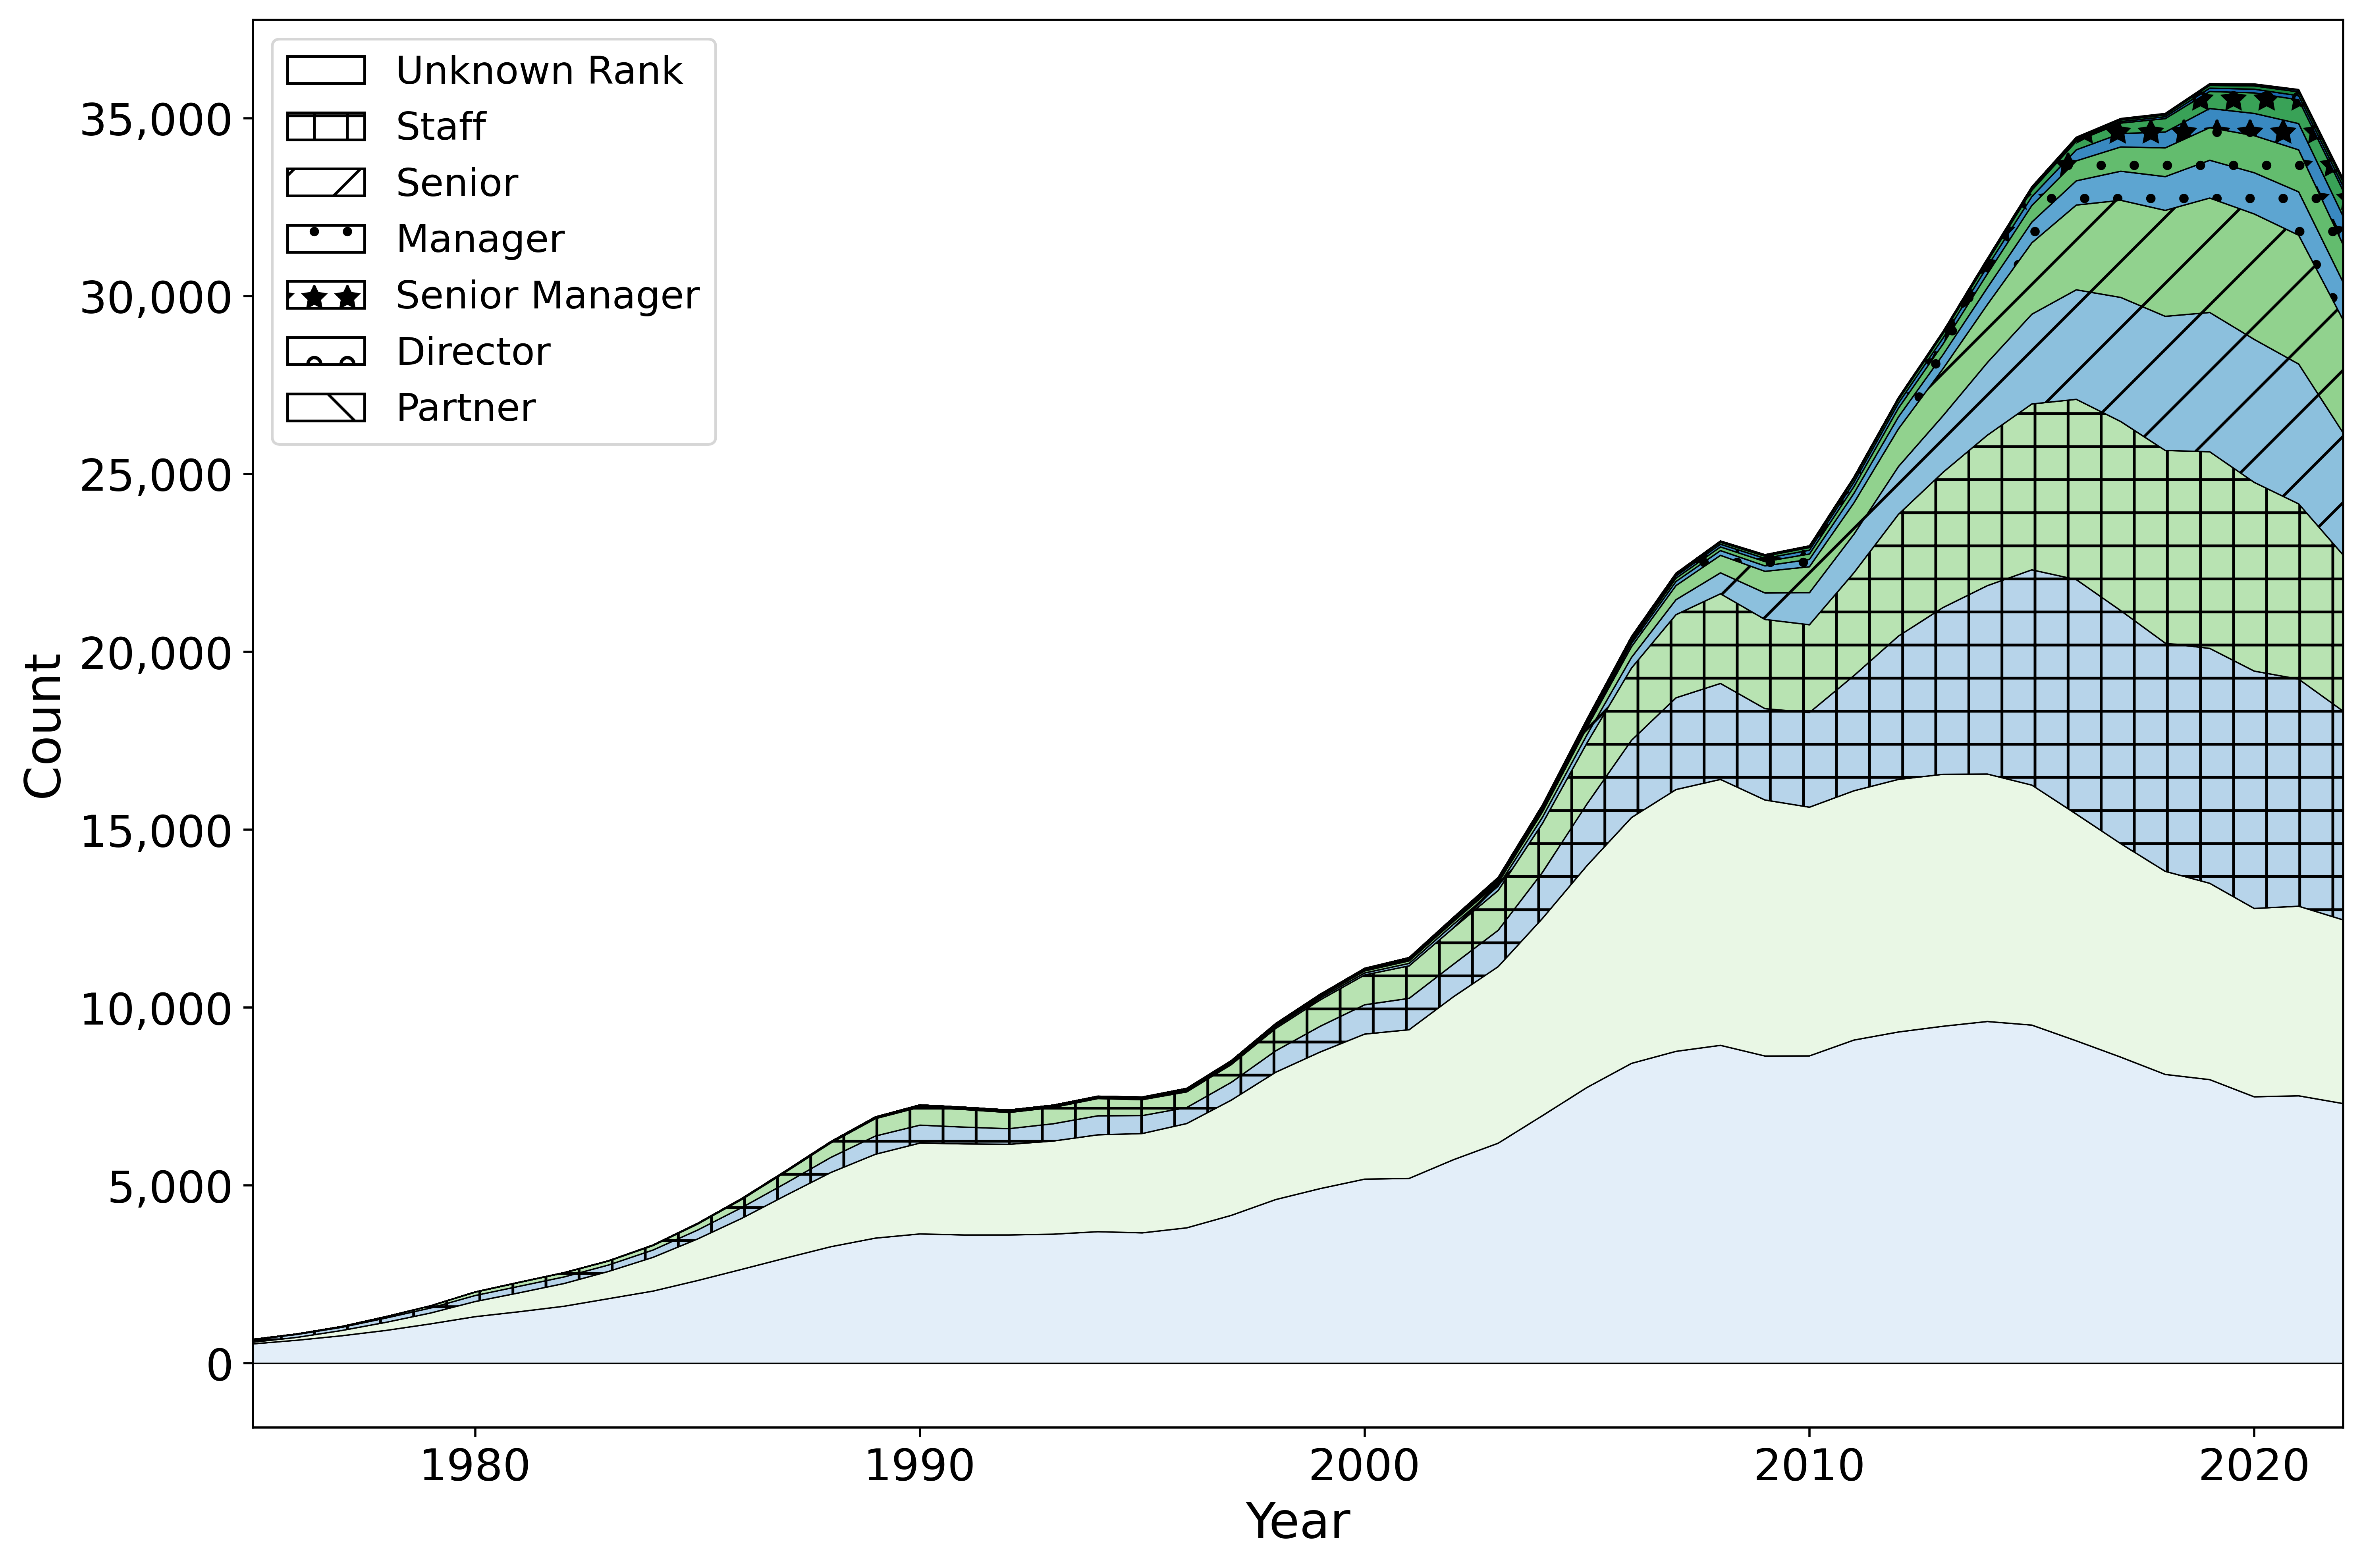
\includegraphics[width=.99\linewidth]{Figures/stackPlot.png}
    \label{figure:stackPlot}
    \footnotesize
    \floatfoot{\textbf{Note}: This figure shows the number of unique Big~4 audit employees in our sample each year, from 1975 through 2023, constructed from Revelio Labs position data. Male auditors are depicted in blue and female auditors in green. Ranks are indicated by the fill pattern as described in the legend.}
\end{figure}

%----- Mechanism Variation -----%
\clearpage
\raggedright
\begin{figure}[t]
    \raggedright
    \captionsetup{labelfont=bf, singlelinecheck=off, justification=raggedright, labelsep=none}
    \caption{: Geographic variation in client-side mechanisms}
    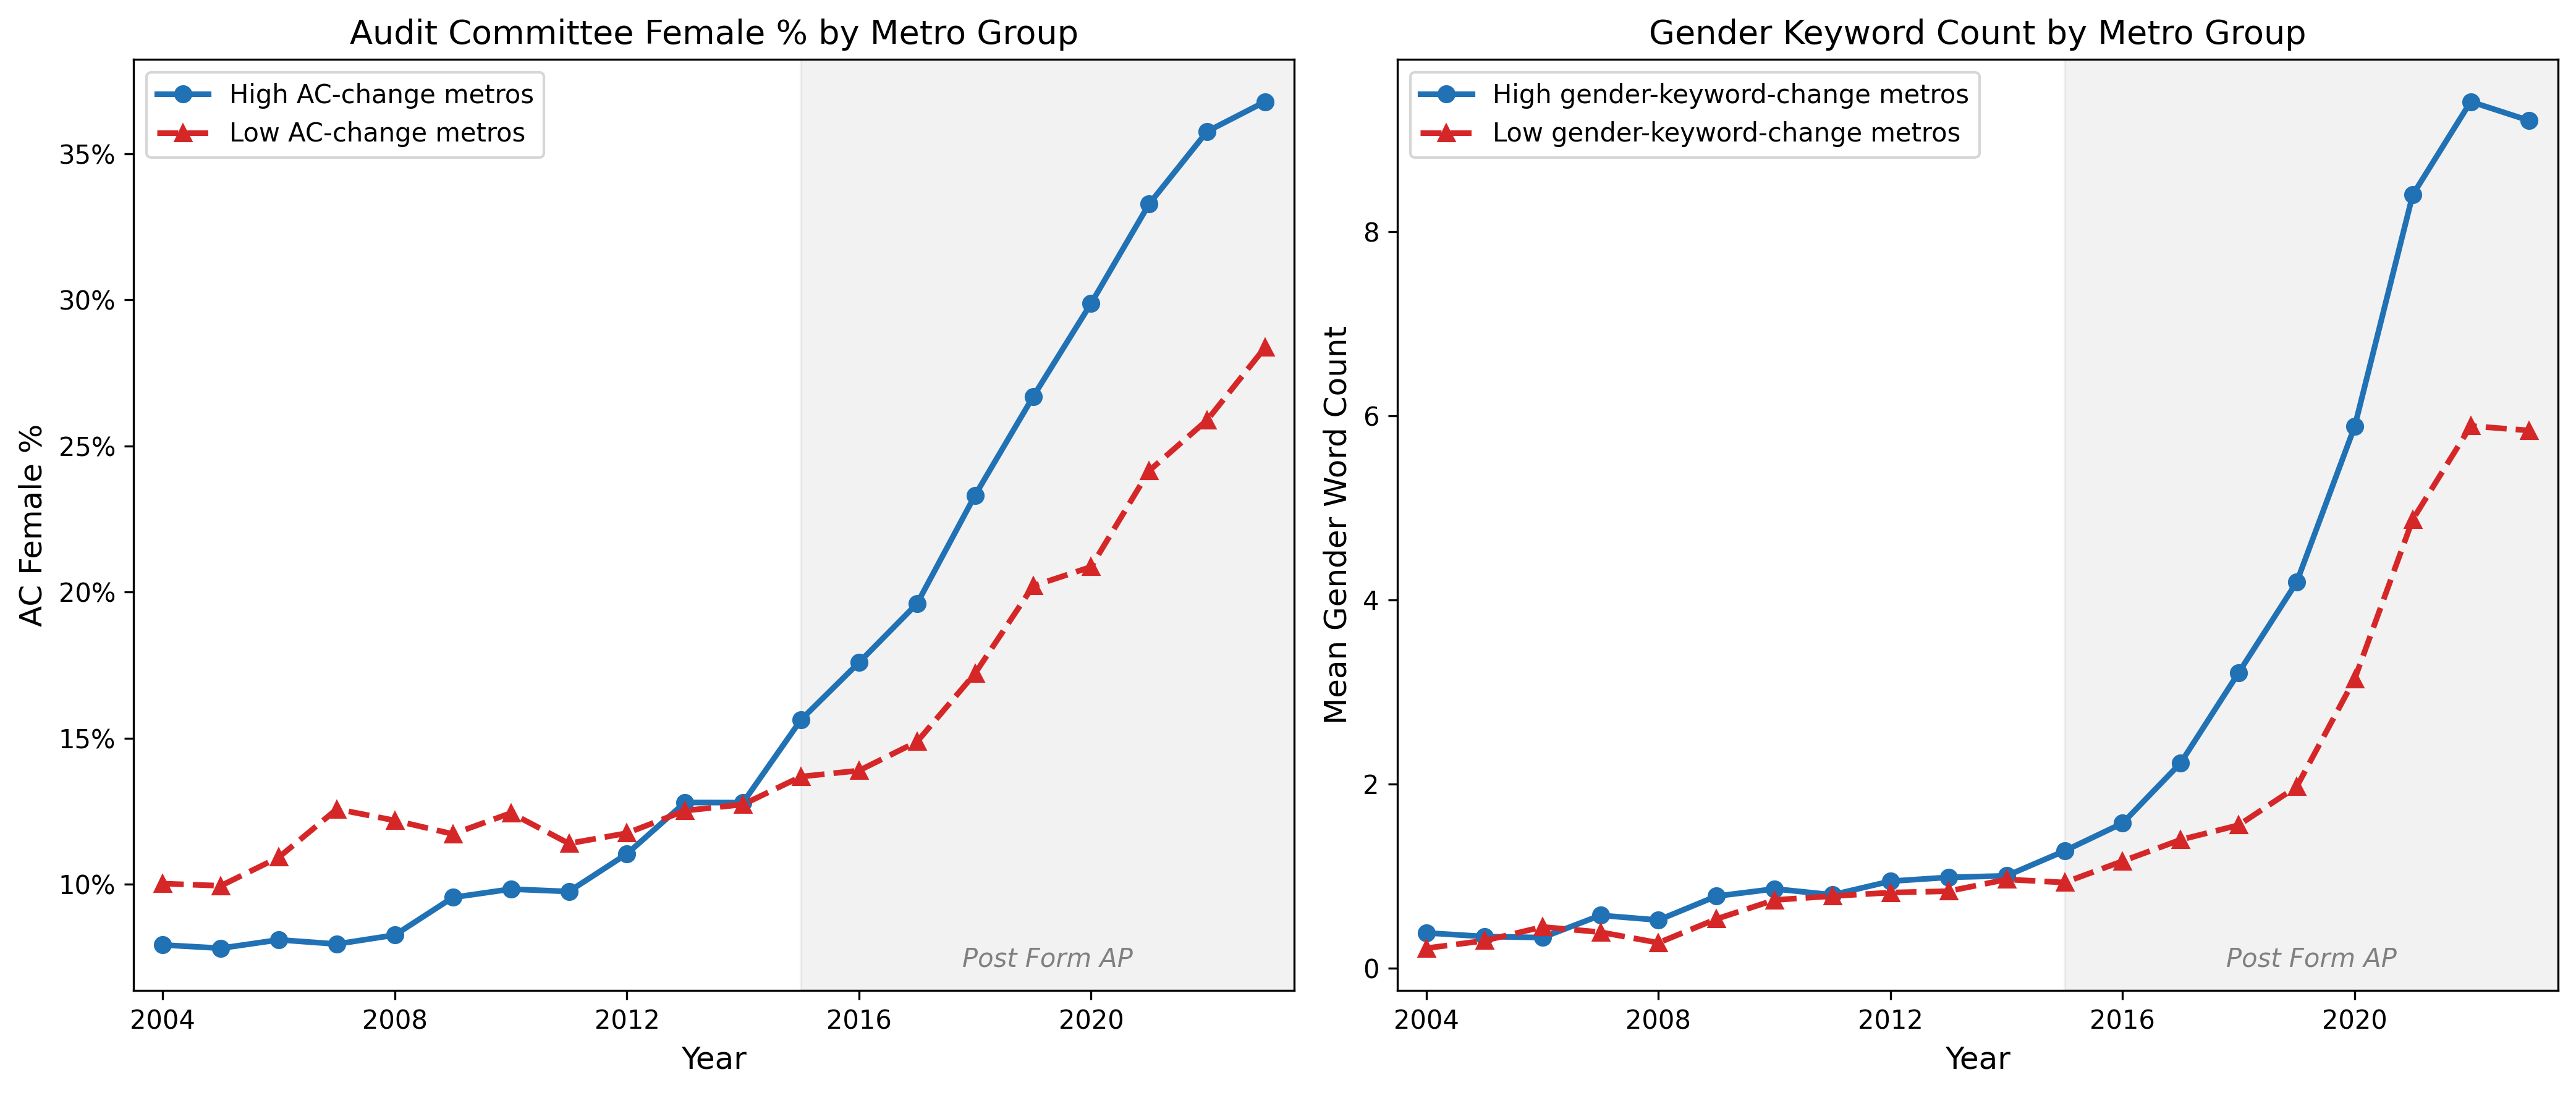
\includegraphics[width=.99\linewidth]{Figures/mechanism_variation_metro.png}
    \label{figure:mechanismVariationMetro}
    \footnotesize
    \floatfoot{\textbf{Note}: This figure plots the time series of two client-side mechanism variables by metropolitan area group. The left panel shows the mean audit committee female percentage; the right panel shows the mean gender keyword count in proxy statements. Metropolitan areas are split into high-change and low-change groups based on the median pre-to-post change in each measure. The shaded region indicates the post-Form~AP period (2015 onward).}
\end{figure}

%----- Retention Gap Map -----%
\begin{figure}[t]
    \raggedright
    \captionsetup{labelfont=bf, singlelinecheck=off, justification=raggedright, labelsep=none}
    \caption{: Female retention advantage by state, pre vs.\ post-Form~AP}
    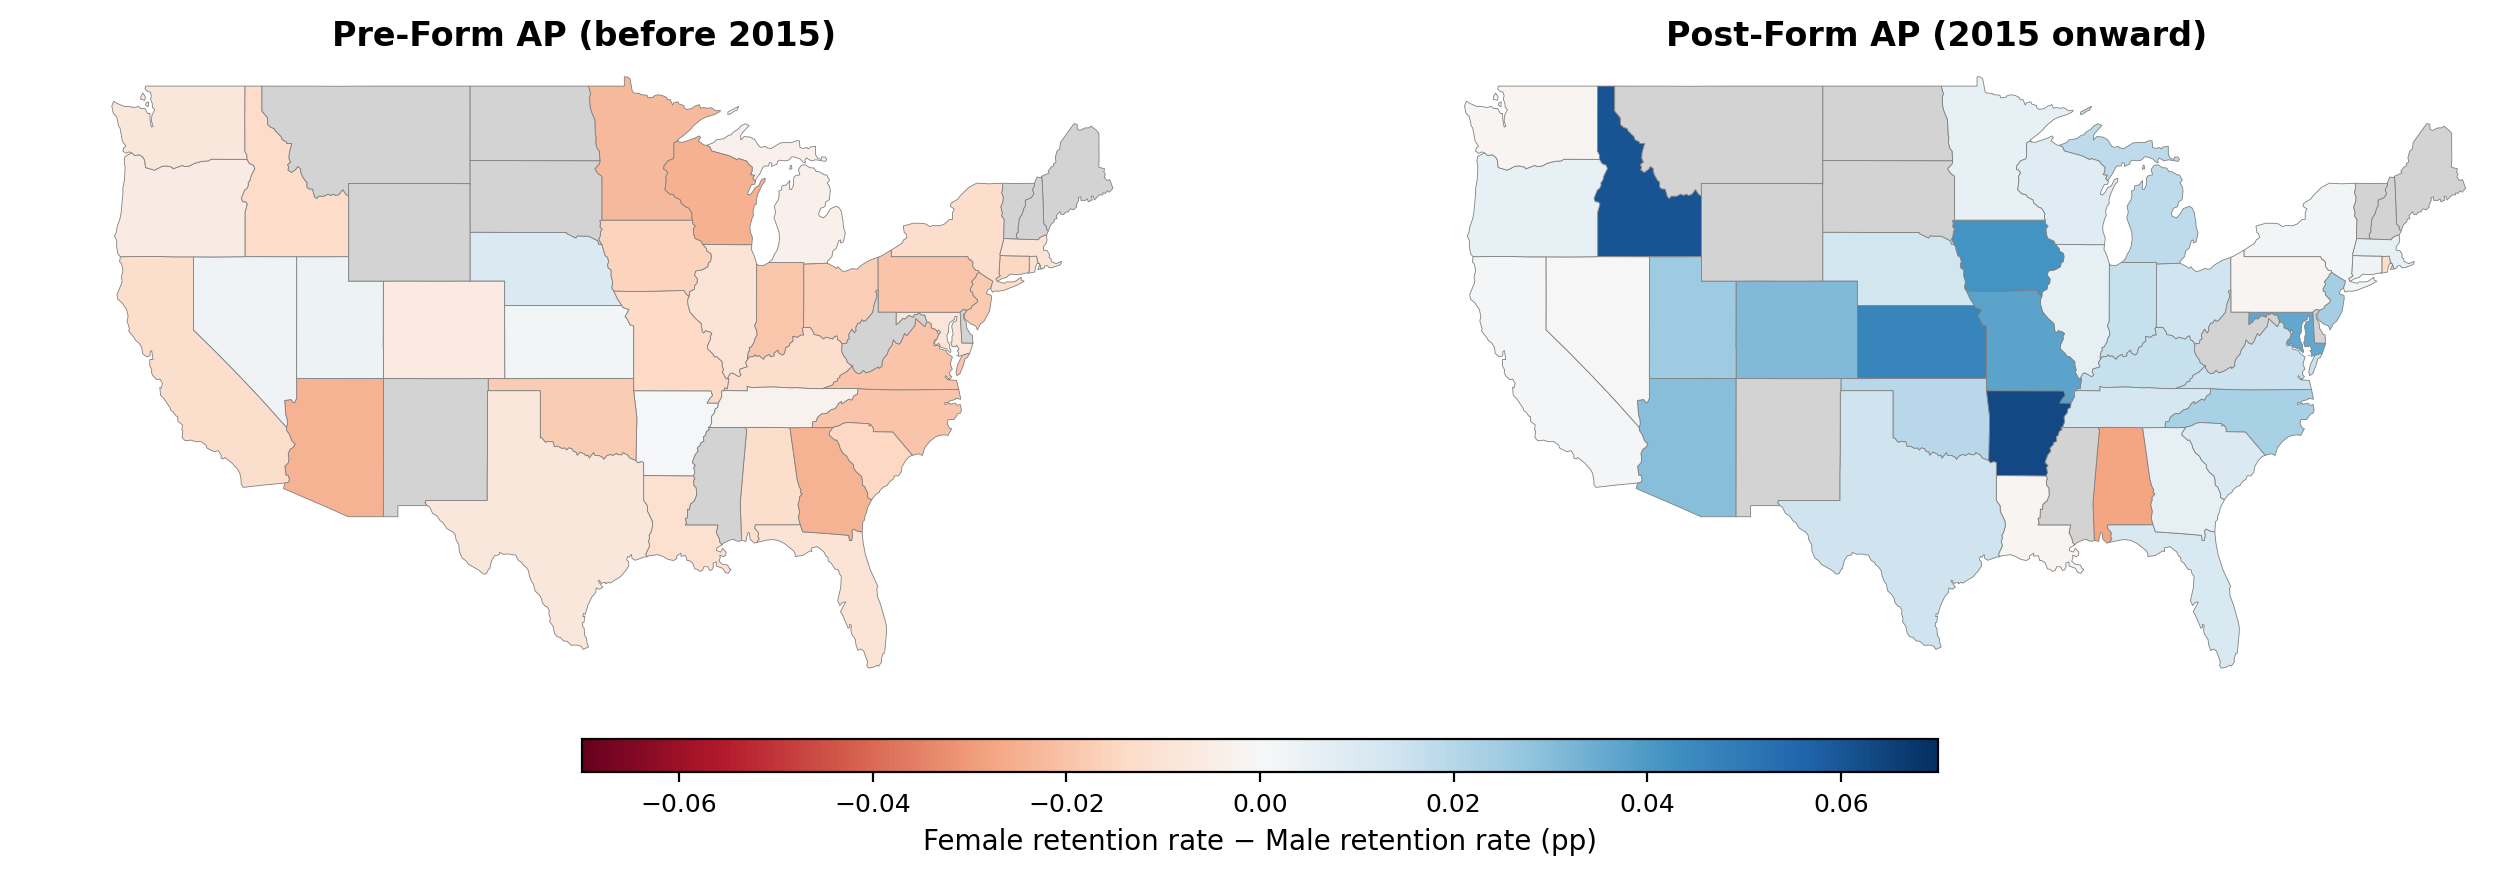
\includegraphics[width=.99\linewidth]{Figures/retentionGapMap.png}
    \label{figure:retentionGapMap}
    \footnotesize
    \floatfoot{\textbf{Note}: This figure shows the difference between female and male auditor retention rates by state, before and after the Form~AP disclosure requirement. Red indicates lower female retention; blue indicates higher female retention. States with fewer than 1,000 Big~4 auditor-year observations are shown in gray. Hawaii meets the inclusion threshold but is not shown on the map.}
\end{figure}

%----- BB5 Investment Banking and Other Financial Services Benchmark -----%
\clearpage
\raggedright
\begin{figure}[t]
    \raggedright
    \captionsetup{labelfont=bf, singlelinecheck=off, justification=raggedright, labelsep=none}
    \caption{: Female retention: investment banking benchmark}
    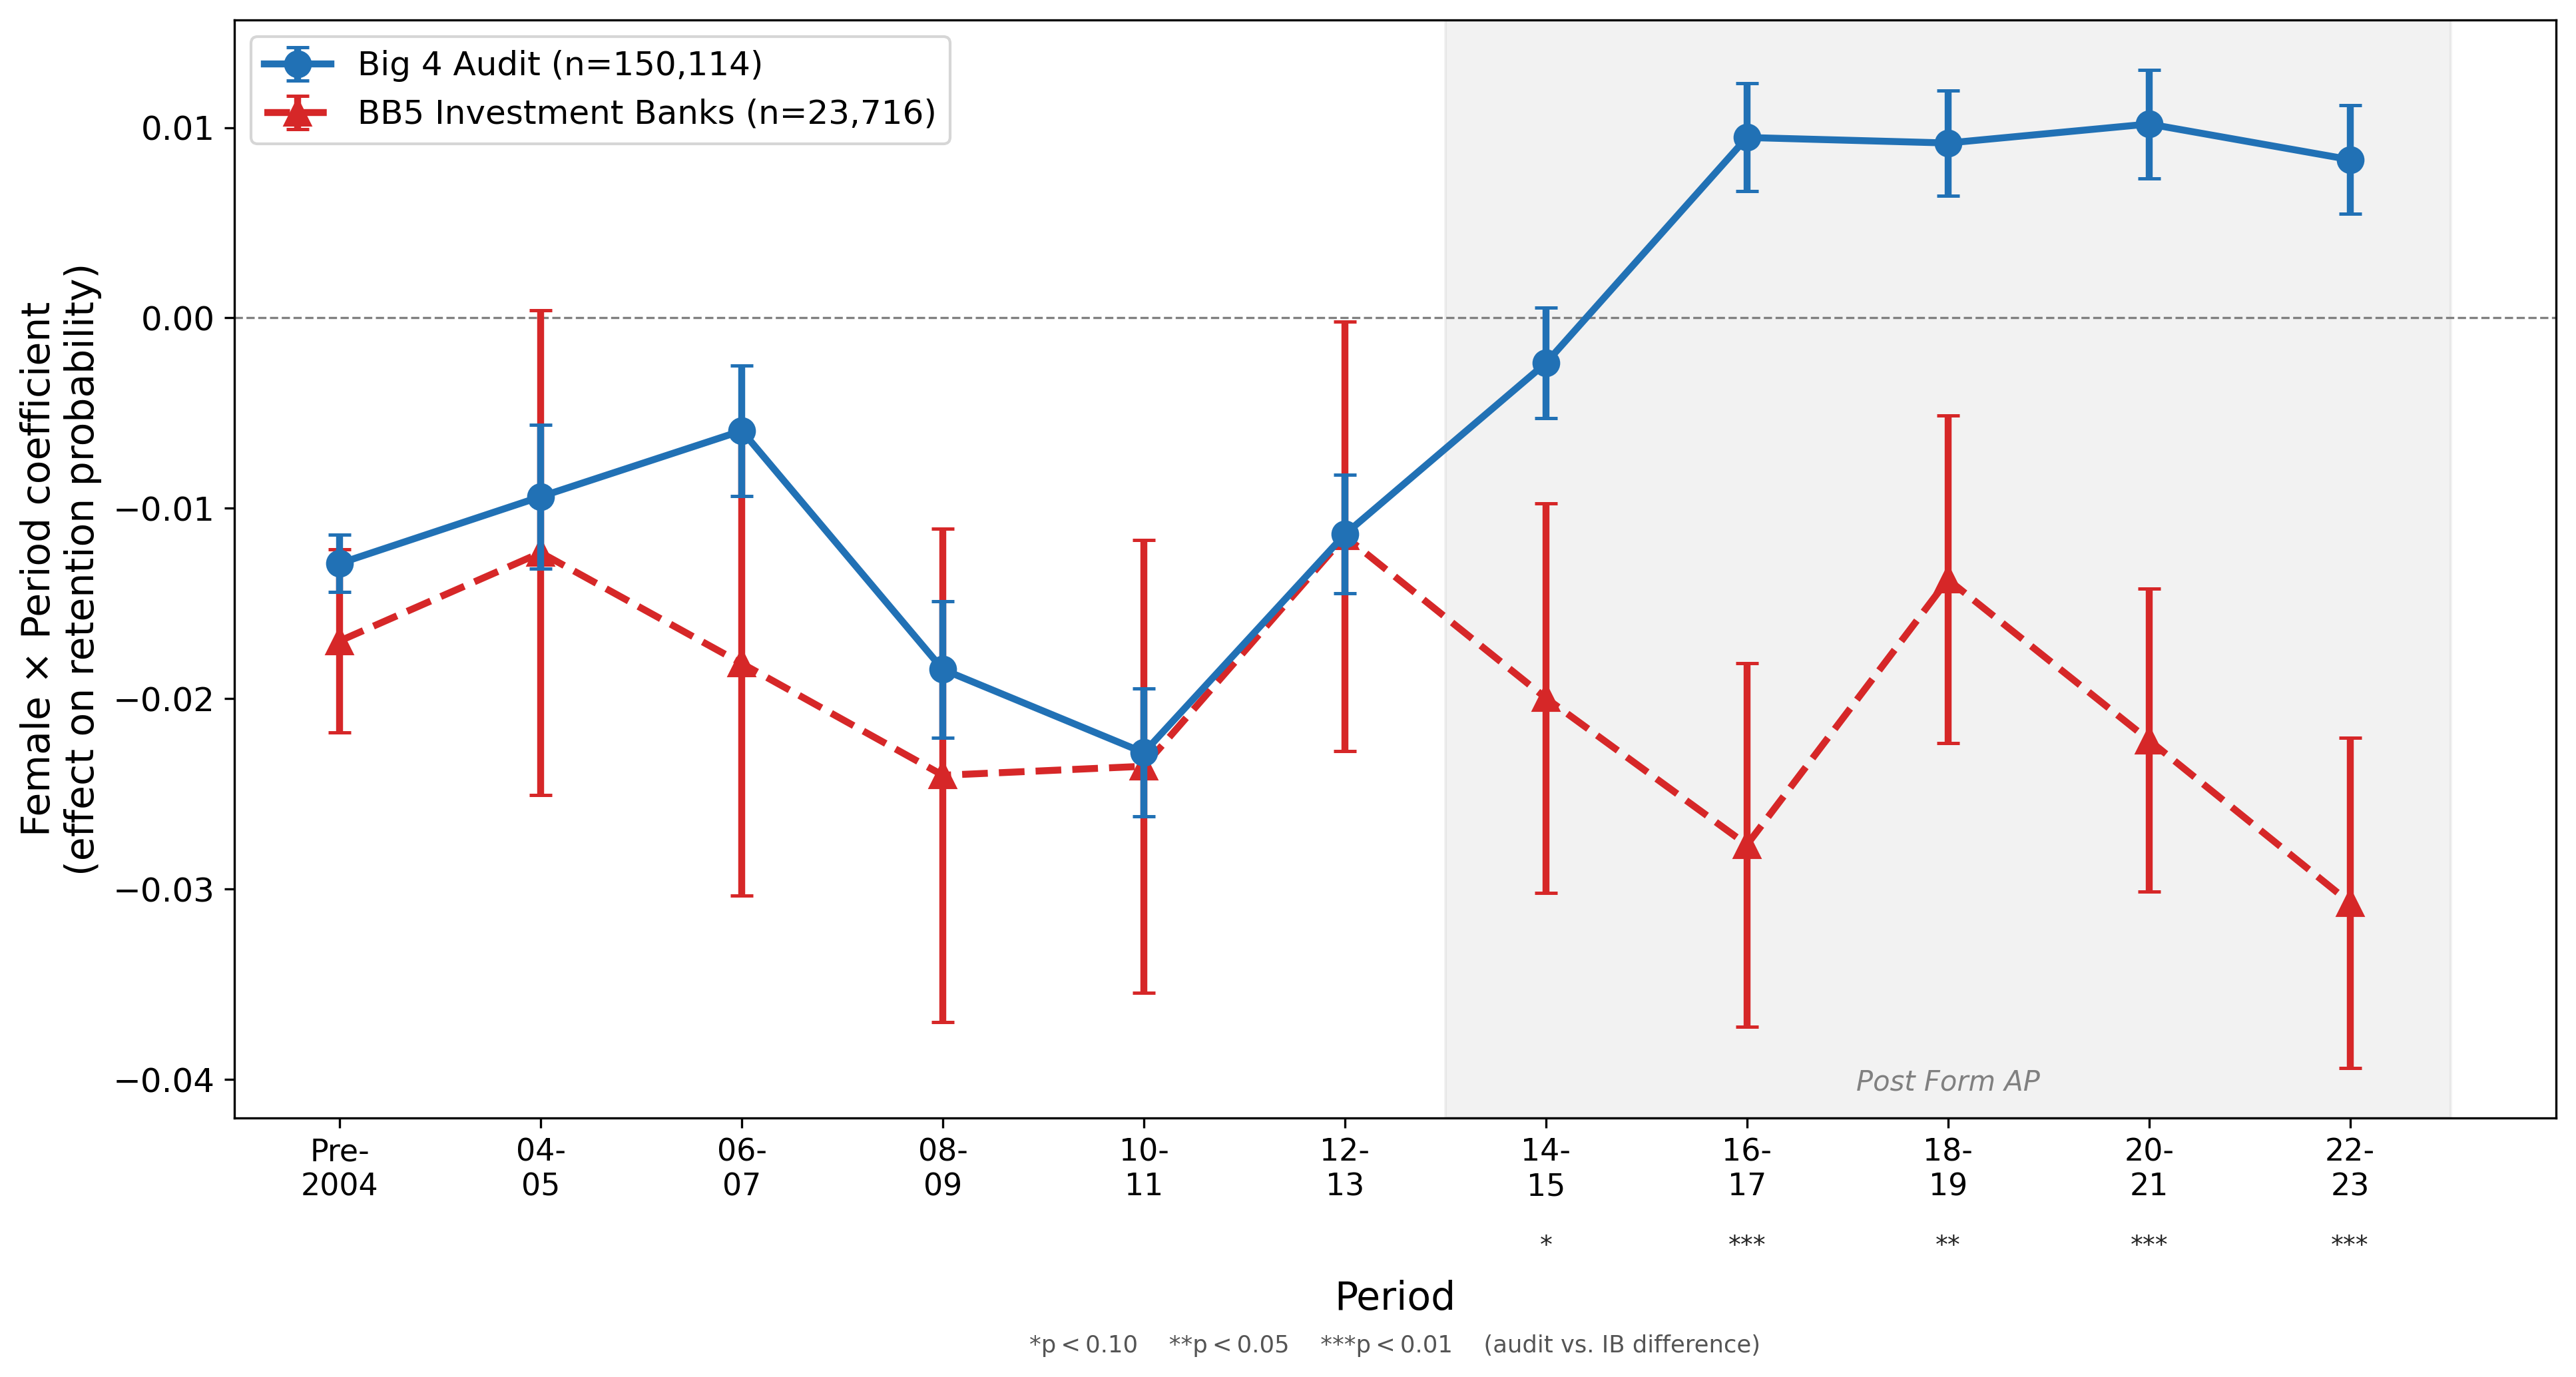
\includegraphics[width=.99\linewidth]{Figures/benchmarkBB5IB.png}
    \label{figure:benchmarkBB5IB}
    \footnotesize
    \floatfoot{\textbf{Note}: This figure plots biennial \textit{Female} $\times$ \textit{Period} coefficients (with standard error bars) from OLS retention models estimated separately on each comparison group. Big~4 Audit (blue) is shown alongside BB5 investment banks (Goldman Sachs, Morgan Stanley, J.P. Morgan, Bank of America, and Citigroup; red). Each model includes employer, calendar-year, and entry-cohort fixed effects, with standard errors clustered by employee. Stars below the x-axis indicate the significance of the difference between Big~4 audit and BB5 investment banking coefficients in each period. The shaded region indicates the post-Form~AP period (2015 onward).}
\end{figure}

%----- OFS Benchmark -----%
\clearpage
\raggedright
\begin{figure}[t]
    \raggedright
    \captionsetup{labelfont=bf, singlelinecheck=off, justification=raggedright, labelsep=none}
    \caption{: Female retention: other financial services benchmark}
    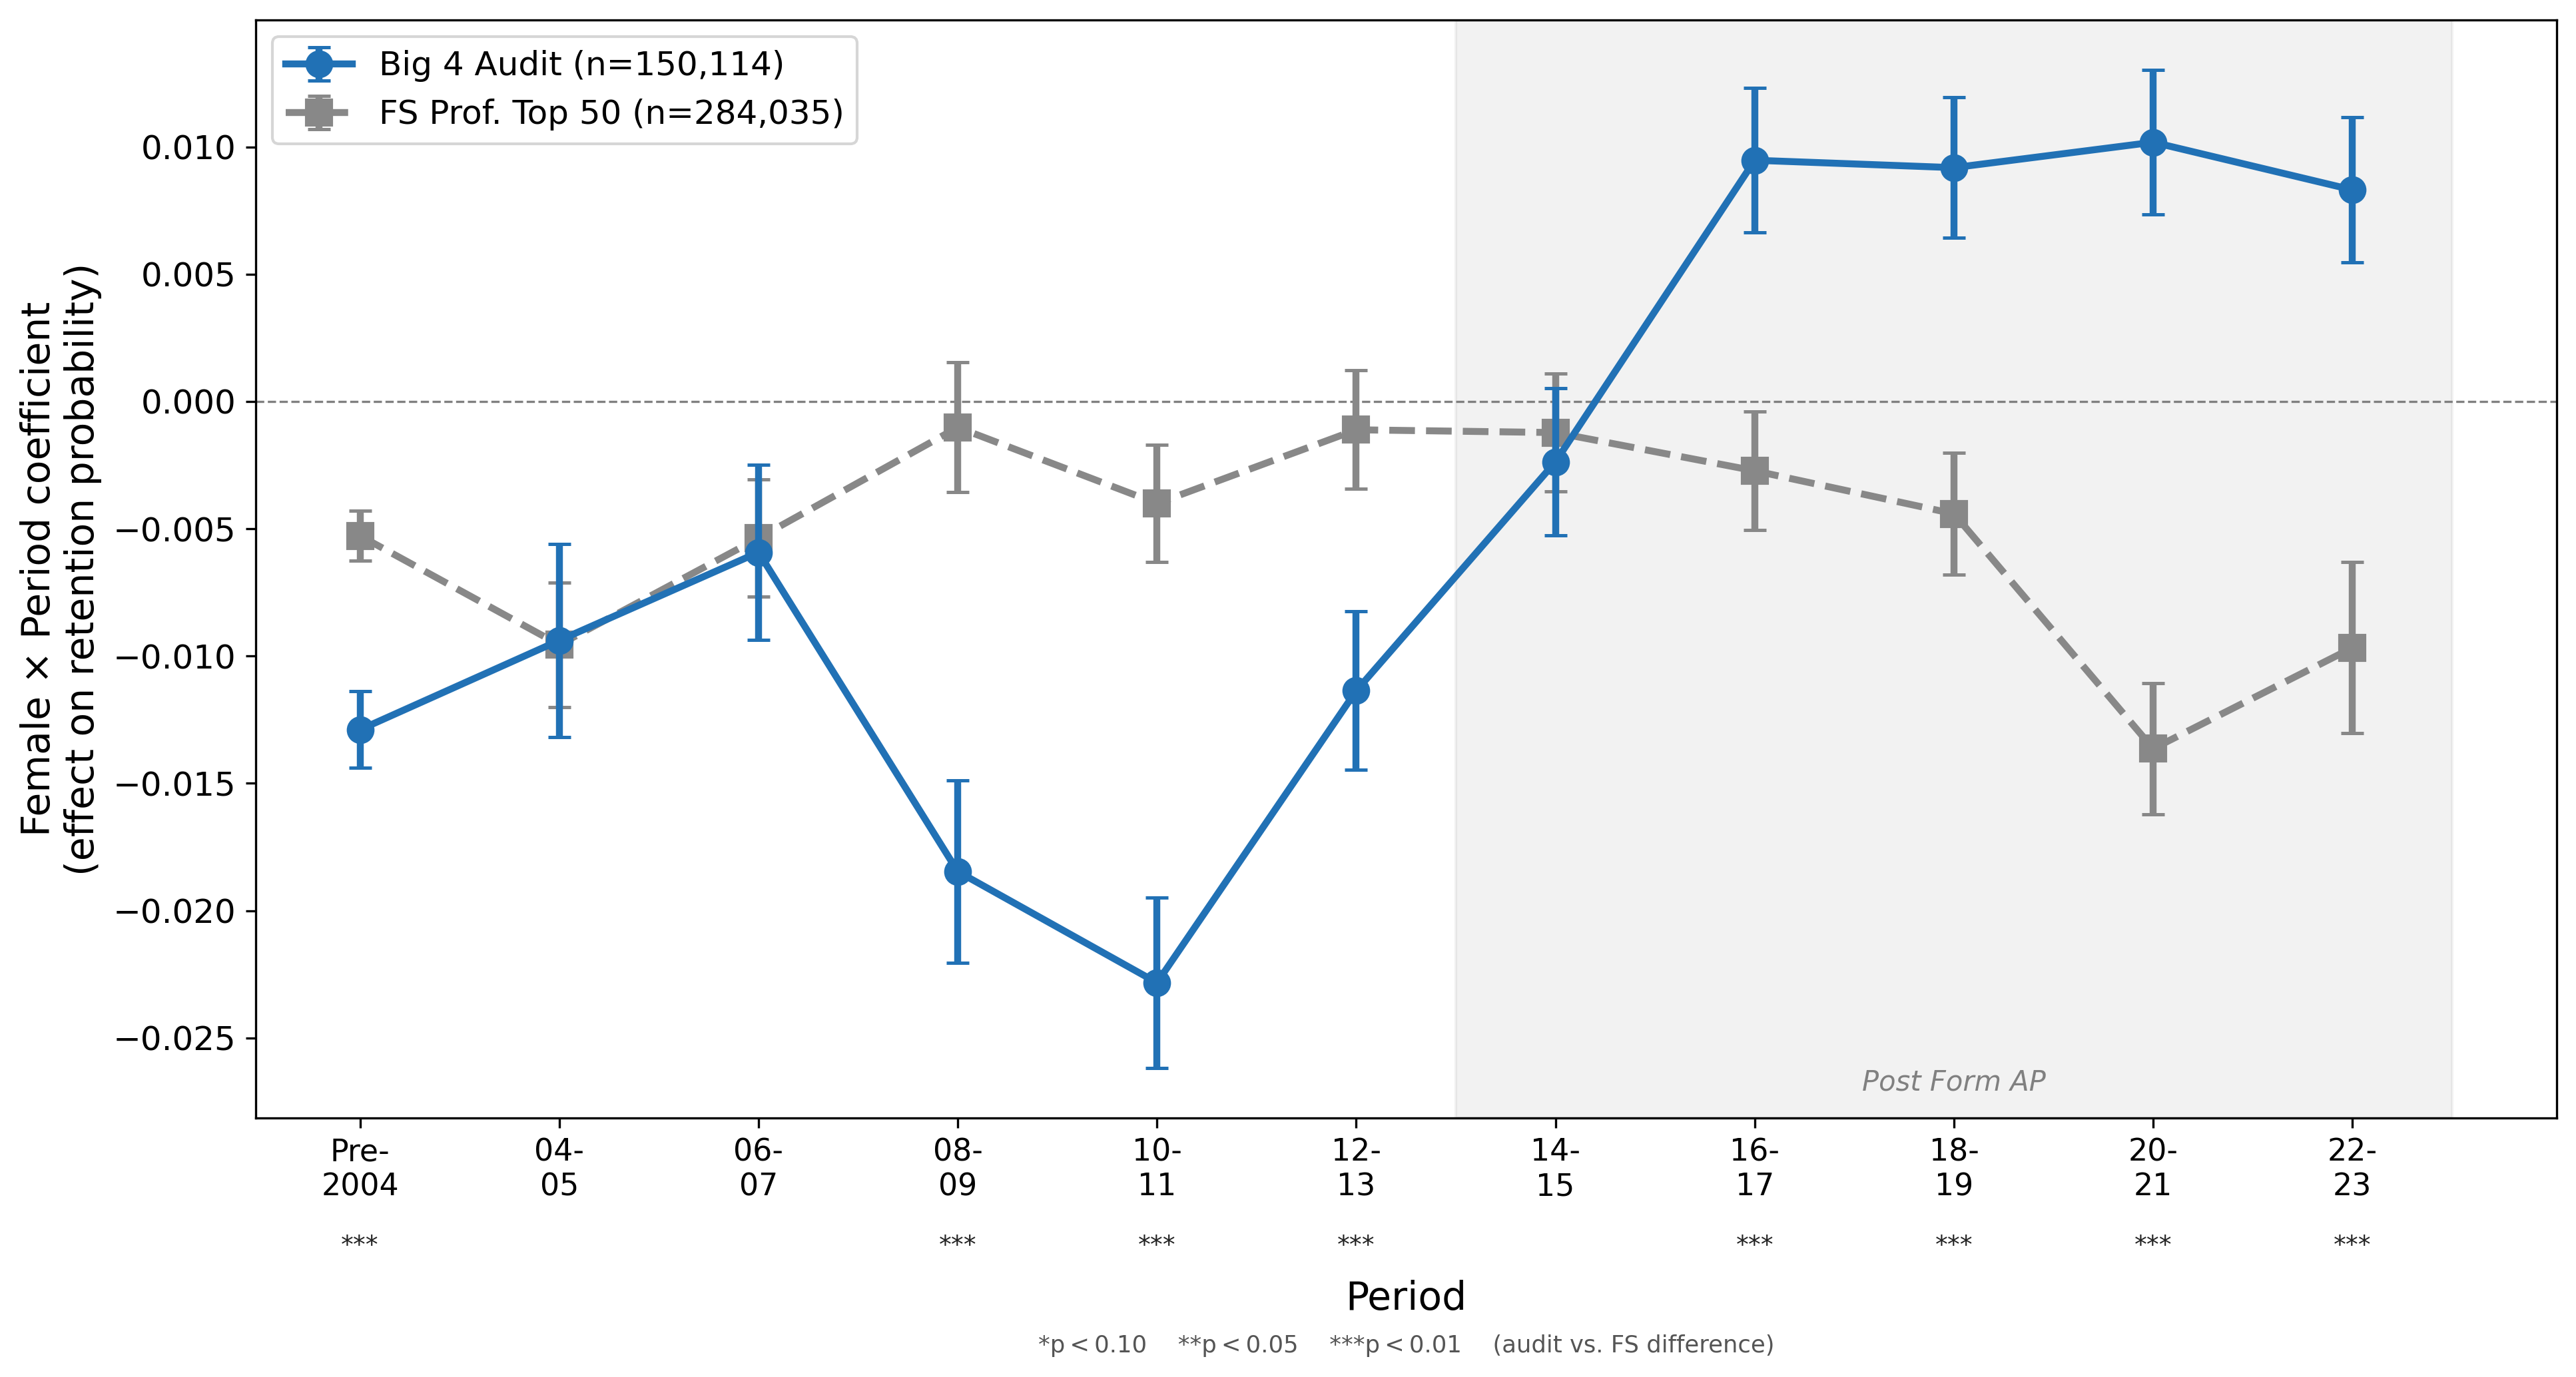
\includegraphics[width=.99\linewidth]{Figures/benchmarkOFS.png}
    \label{figure:benchmarkOFS}
    \footnotesize
    \floatfoot{\textbf{Note}: This figure plots biennial \textit{Female} $\times$ \textit{Period} coefficients (with standard error bars) from OLS retention models estimated separately on each comparison group. Big~4 Audit (blue) is shown alongside professionals at the 50 largest financial services firms excluding accounting firms (gray). Each model includes employer, calendar-year, and entry-cohort fixed effects, with standard errors clustered by employee. Stars below the x-axis indicate the significance of the difference between Big~4 audit and OFS coefficients in each period. The shaded region indicates the post-Form~AP period (2015 onward).}
\end{figure}

%----- Non-B4 Audit Firm Benchmarks + Big 4 Tax -----%
\clearpage
\raggedright
\begin{figure}[t]
    \raggedright
    \captionsetup{labelfont=bf, singlelinecheck=off, justification=raggedright, labelsep=none}
    \caption{: Non-Big 4 audit firm benchmarks}
    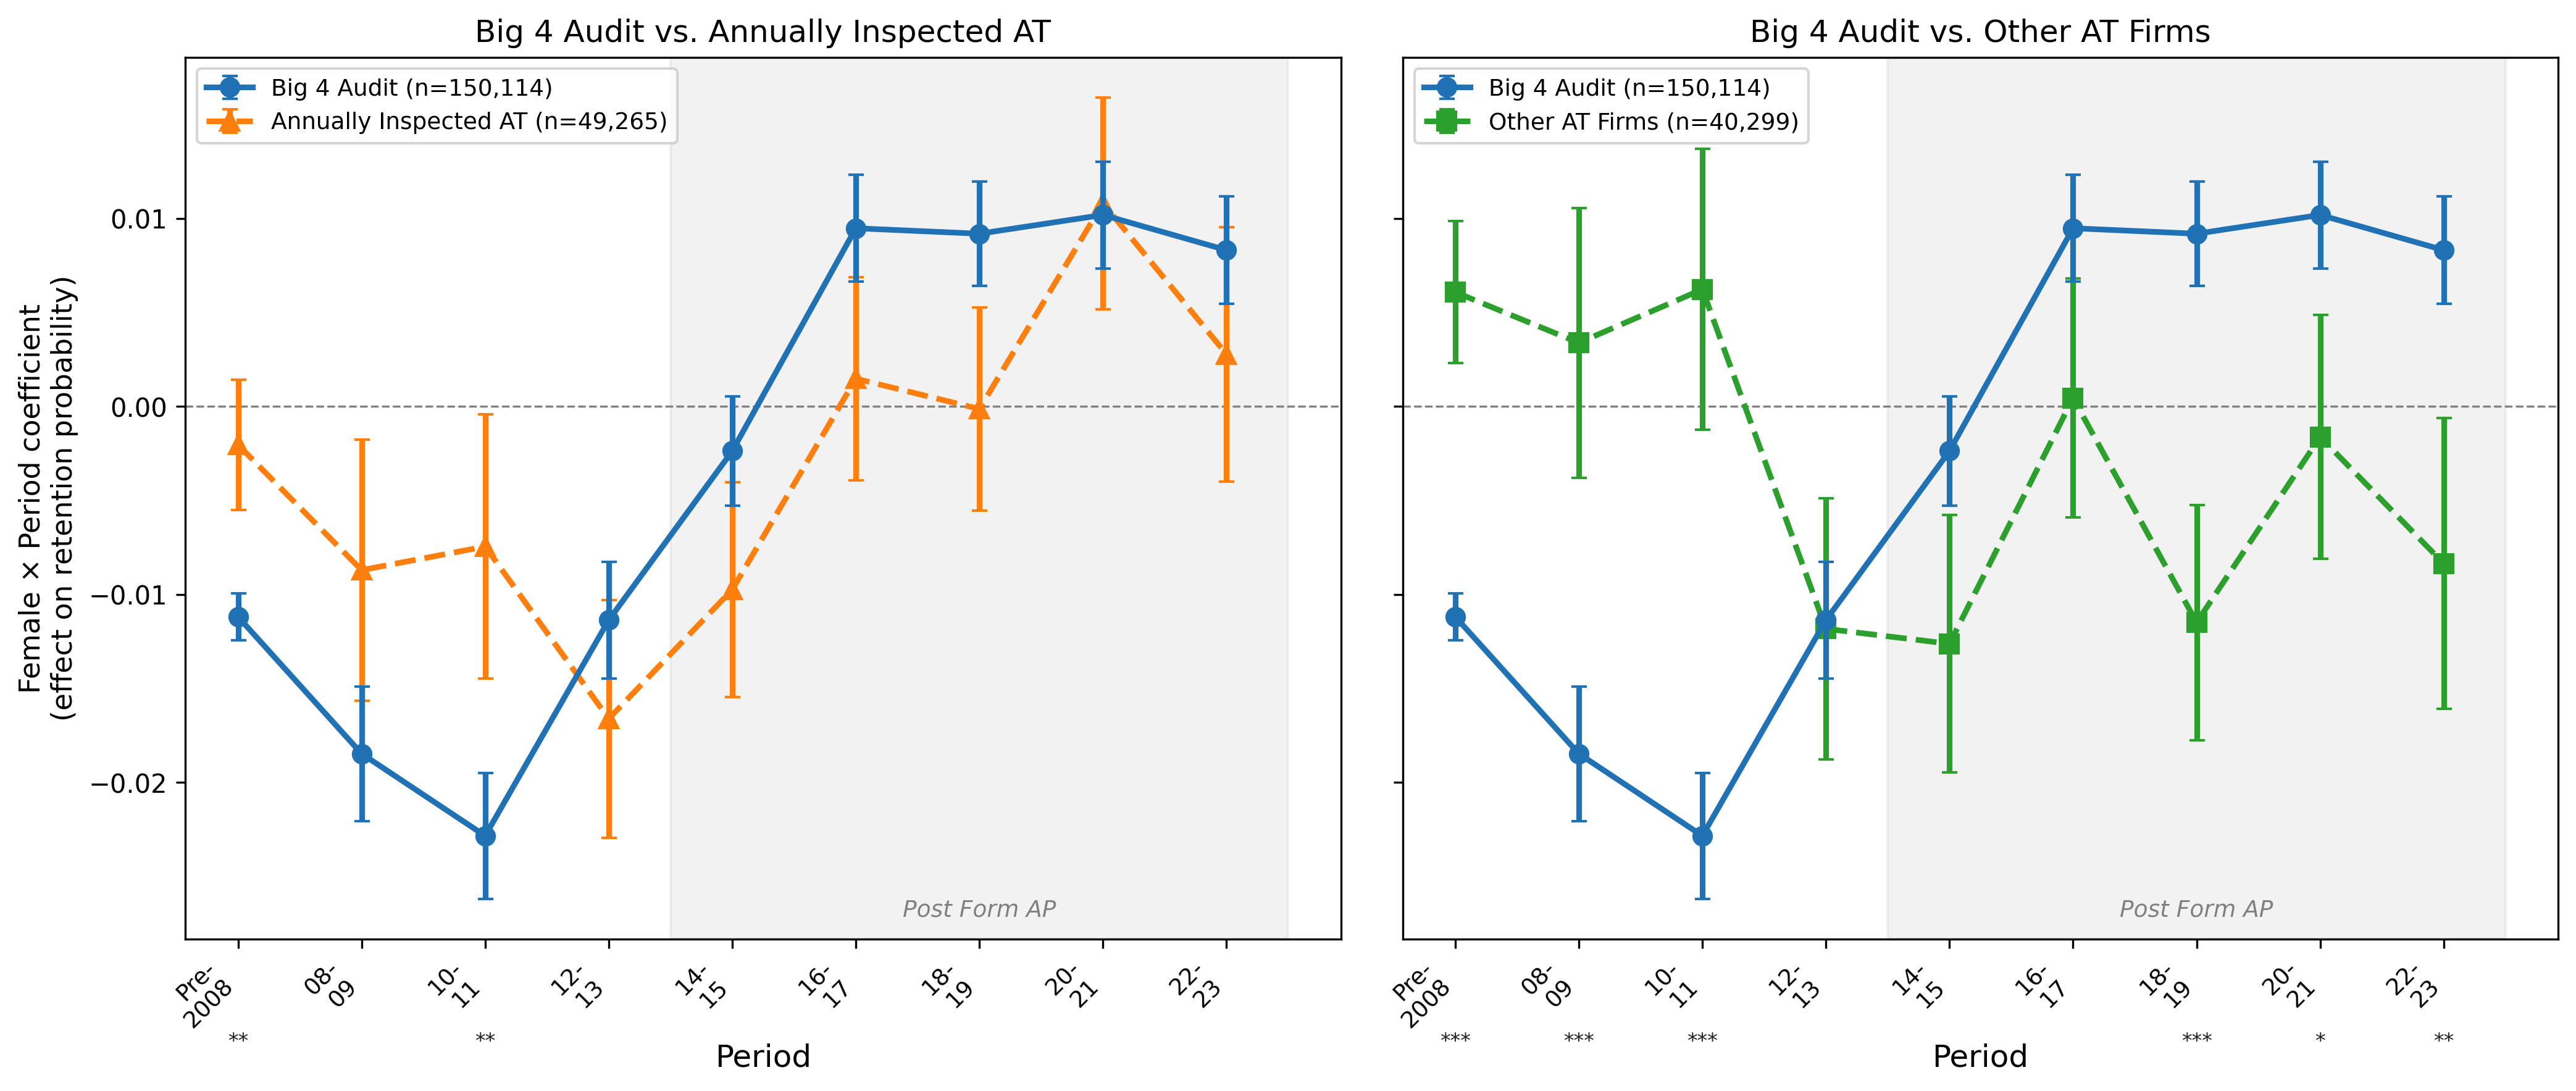
\includegraphics[width=.99\linewidth]{Figures/benchmarkATCombined.png}
    \label{figure:benchmarkATCombined}
    \footnotesize
    \floatfoot{\textbf{Note}: This figure plots biennial \textit{Female} $\times$ \textit{Period} coefficients (with standard error bars) from OLS retention models estimated on Big~4 auditors (blue) alongside two non-Big~4 audit firm benchmarks. Non-Big~4 firms are drawn from the \textit{Accounting Today} Top~100 firms list. The left panel compares Big~4 audit to annually inspected firms (Grant Thornton, BDO, RSM, Crowe, Forvis, Moss Adams, Baker Tilly). The right panel compares Big~4 audit to other (non-annually inspected) firms. Stars below the x-axis indicate the significance of the difference between the Big~4 audit and benchmark coefficients in each period. The shaded region indicates the post-Form~AP period (2015 onward).}
\end{figure}

\begin{figure}[t]
    \raggedright
    \captionsetup{labelfont=bf, singlelinecheck=off, justification=raggedright, labelsep=none}
    \caption{: Female retention: Big 4 tax divisions}
    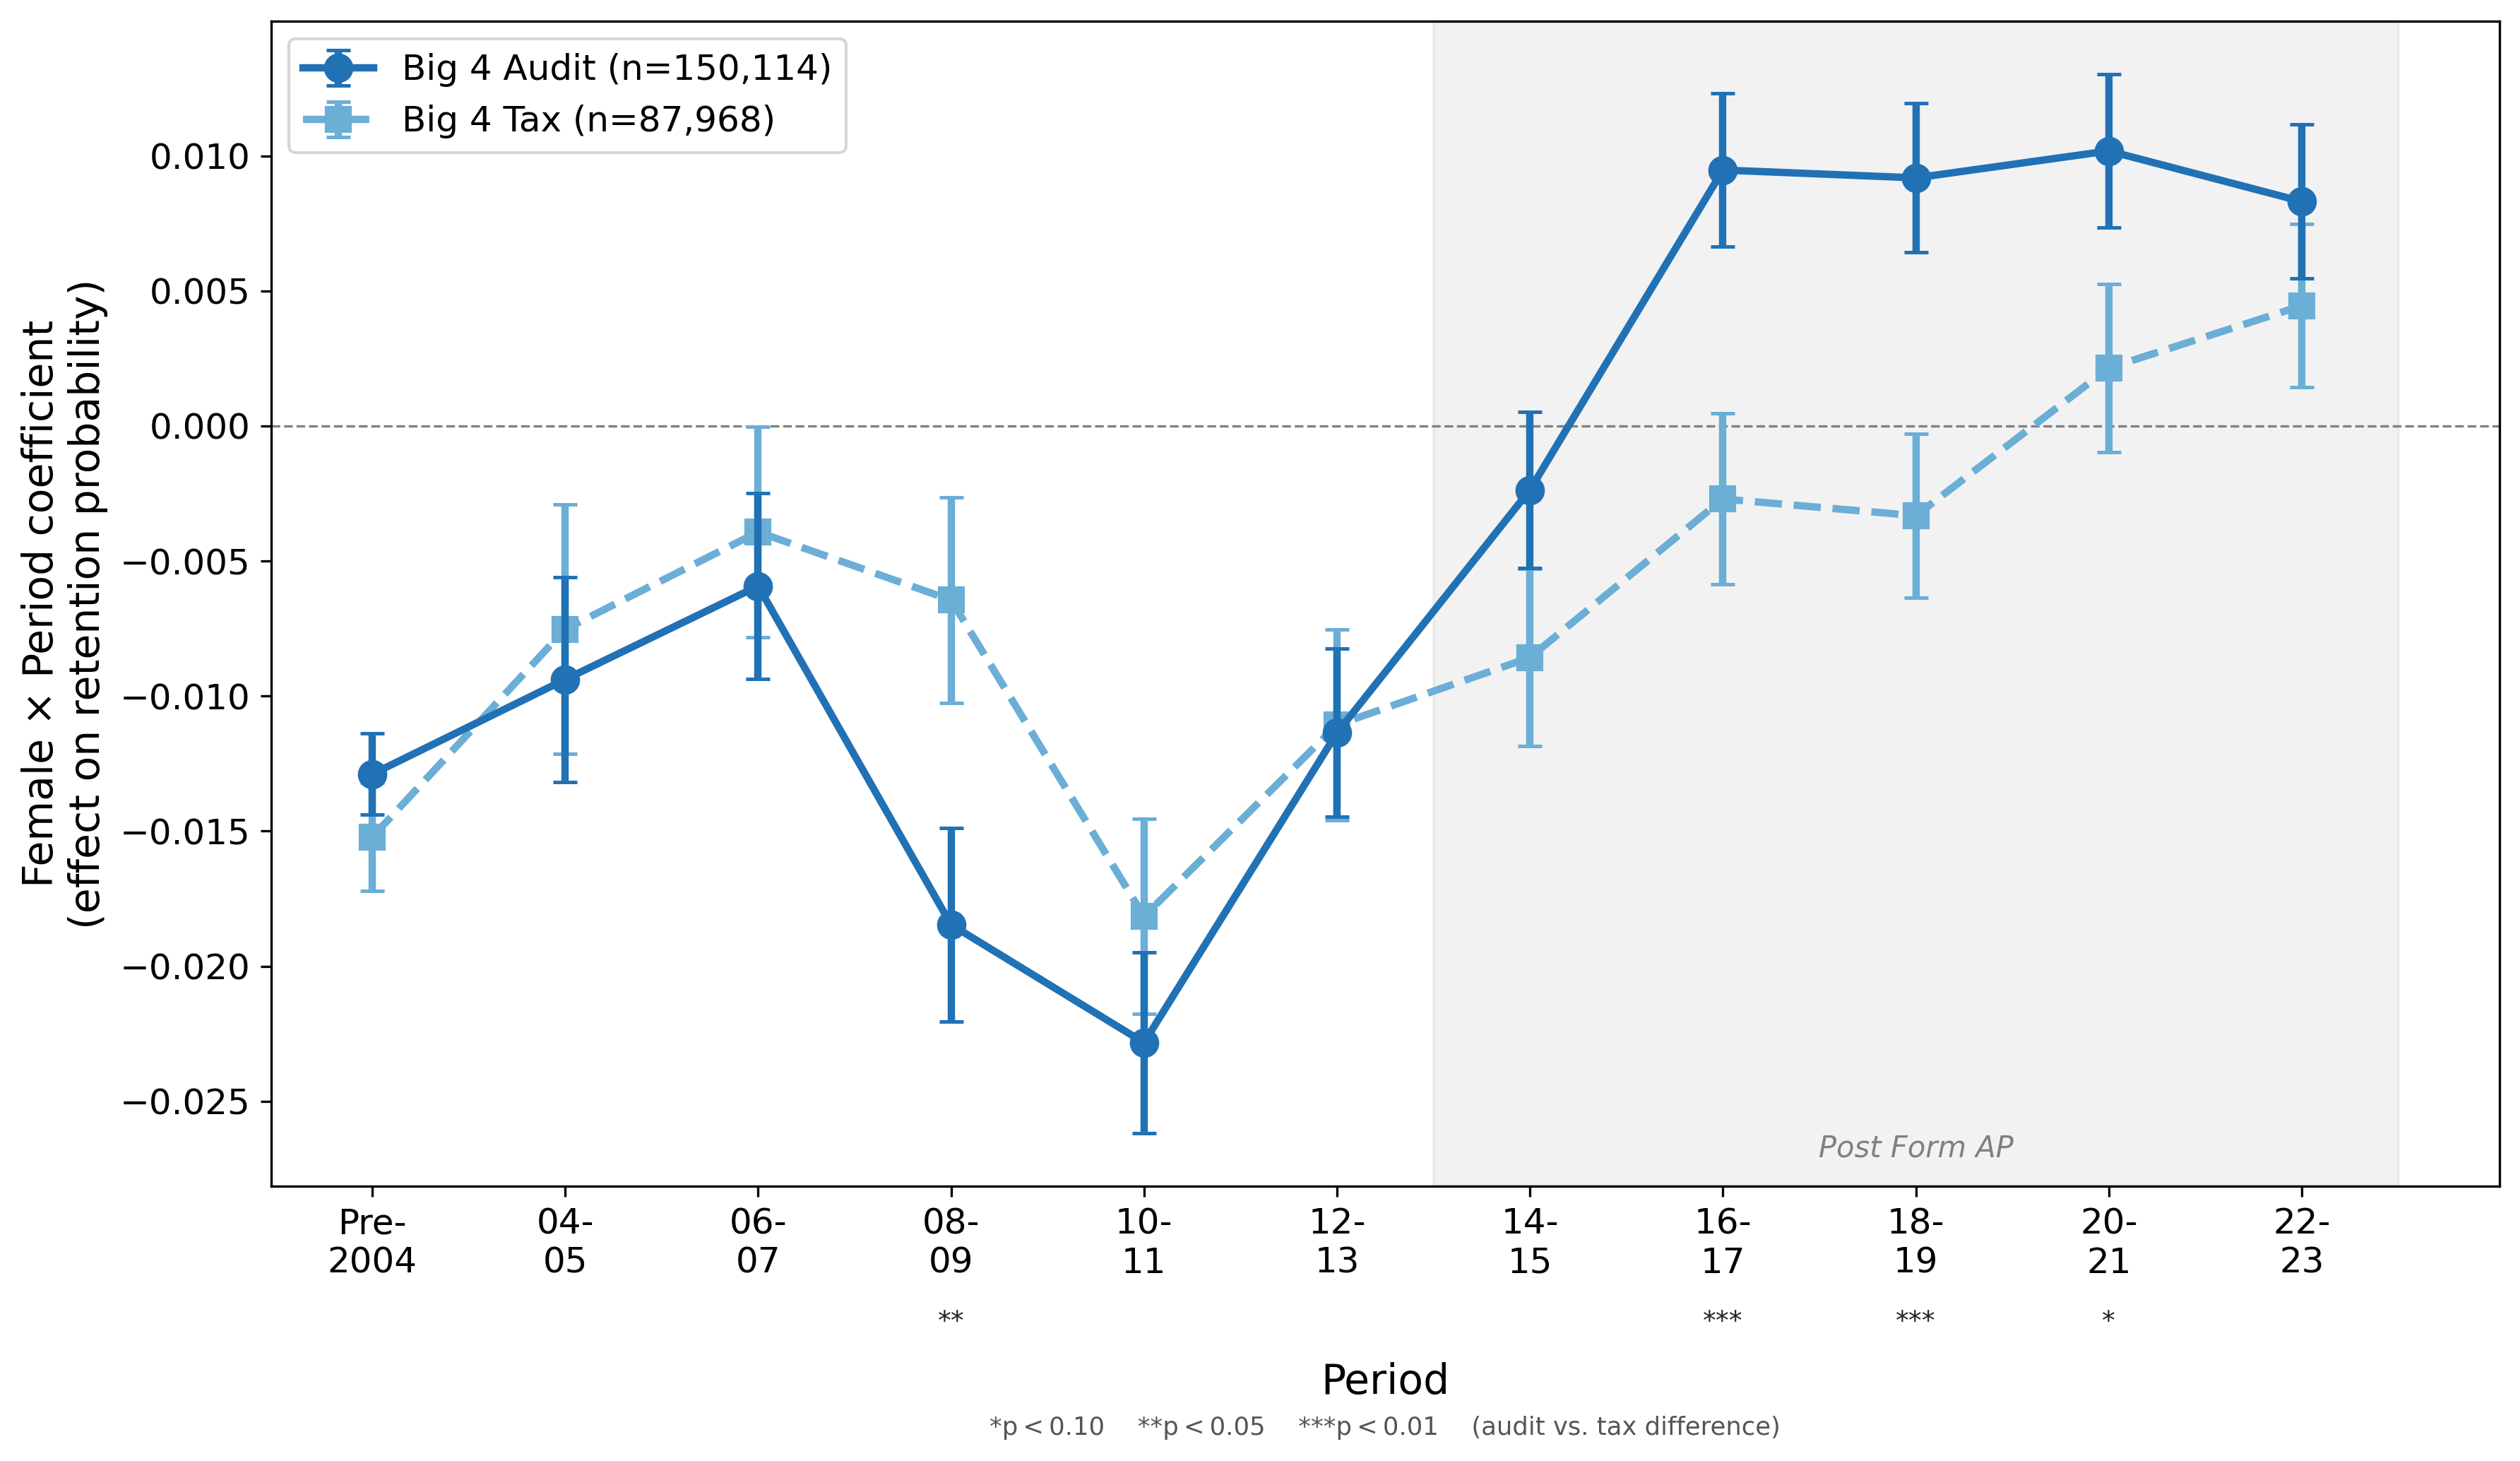
\includegraphics[width=.99\linewidth]{Figures/benchmarkB4Tax.png}
    \label{figure:benchmarkB4Tax}
    \footnotesize
    \floatfoot{\textbf{Note}: This figure plots biennial \textit{Female} $\times$ \textit{Period} coefficients (with standard error bars) from OLS retention models estimated on Big~4 auditors (blue) alongside Big~4 tax professionals. Tax employees share the same firms, offices, and HR policies as Big~4 auditors but are not directly subject to the Form~AP disclosure requirement, making this an internal benchmark for audit-specific effects. The shaded region indicates the post-Form~AP period (2015 onward).}
\end{figure}

%----- Supply vs Entry -----%
\clearpage
\raggedright
\begin{figure}[t]
    \raggedright
    \captionsetup{labelfont=bf, singlelinecheck=off, justification=raggedright, labelsep=none}
    \caption{: Gender composition of accounting talent pipeline vs.\ Big~4 audit new hires}
    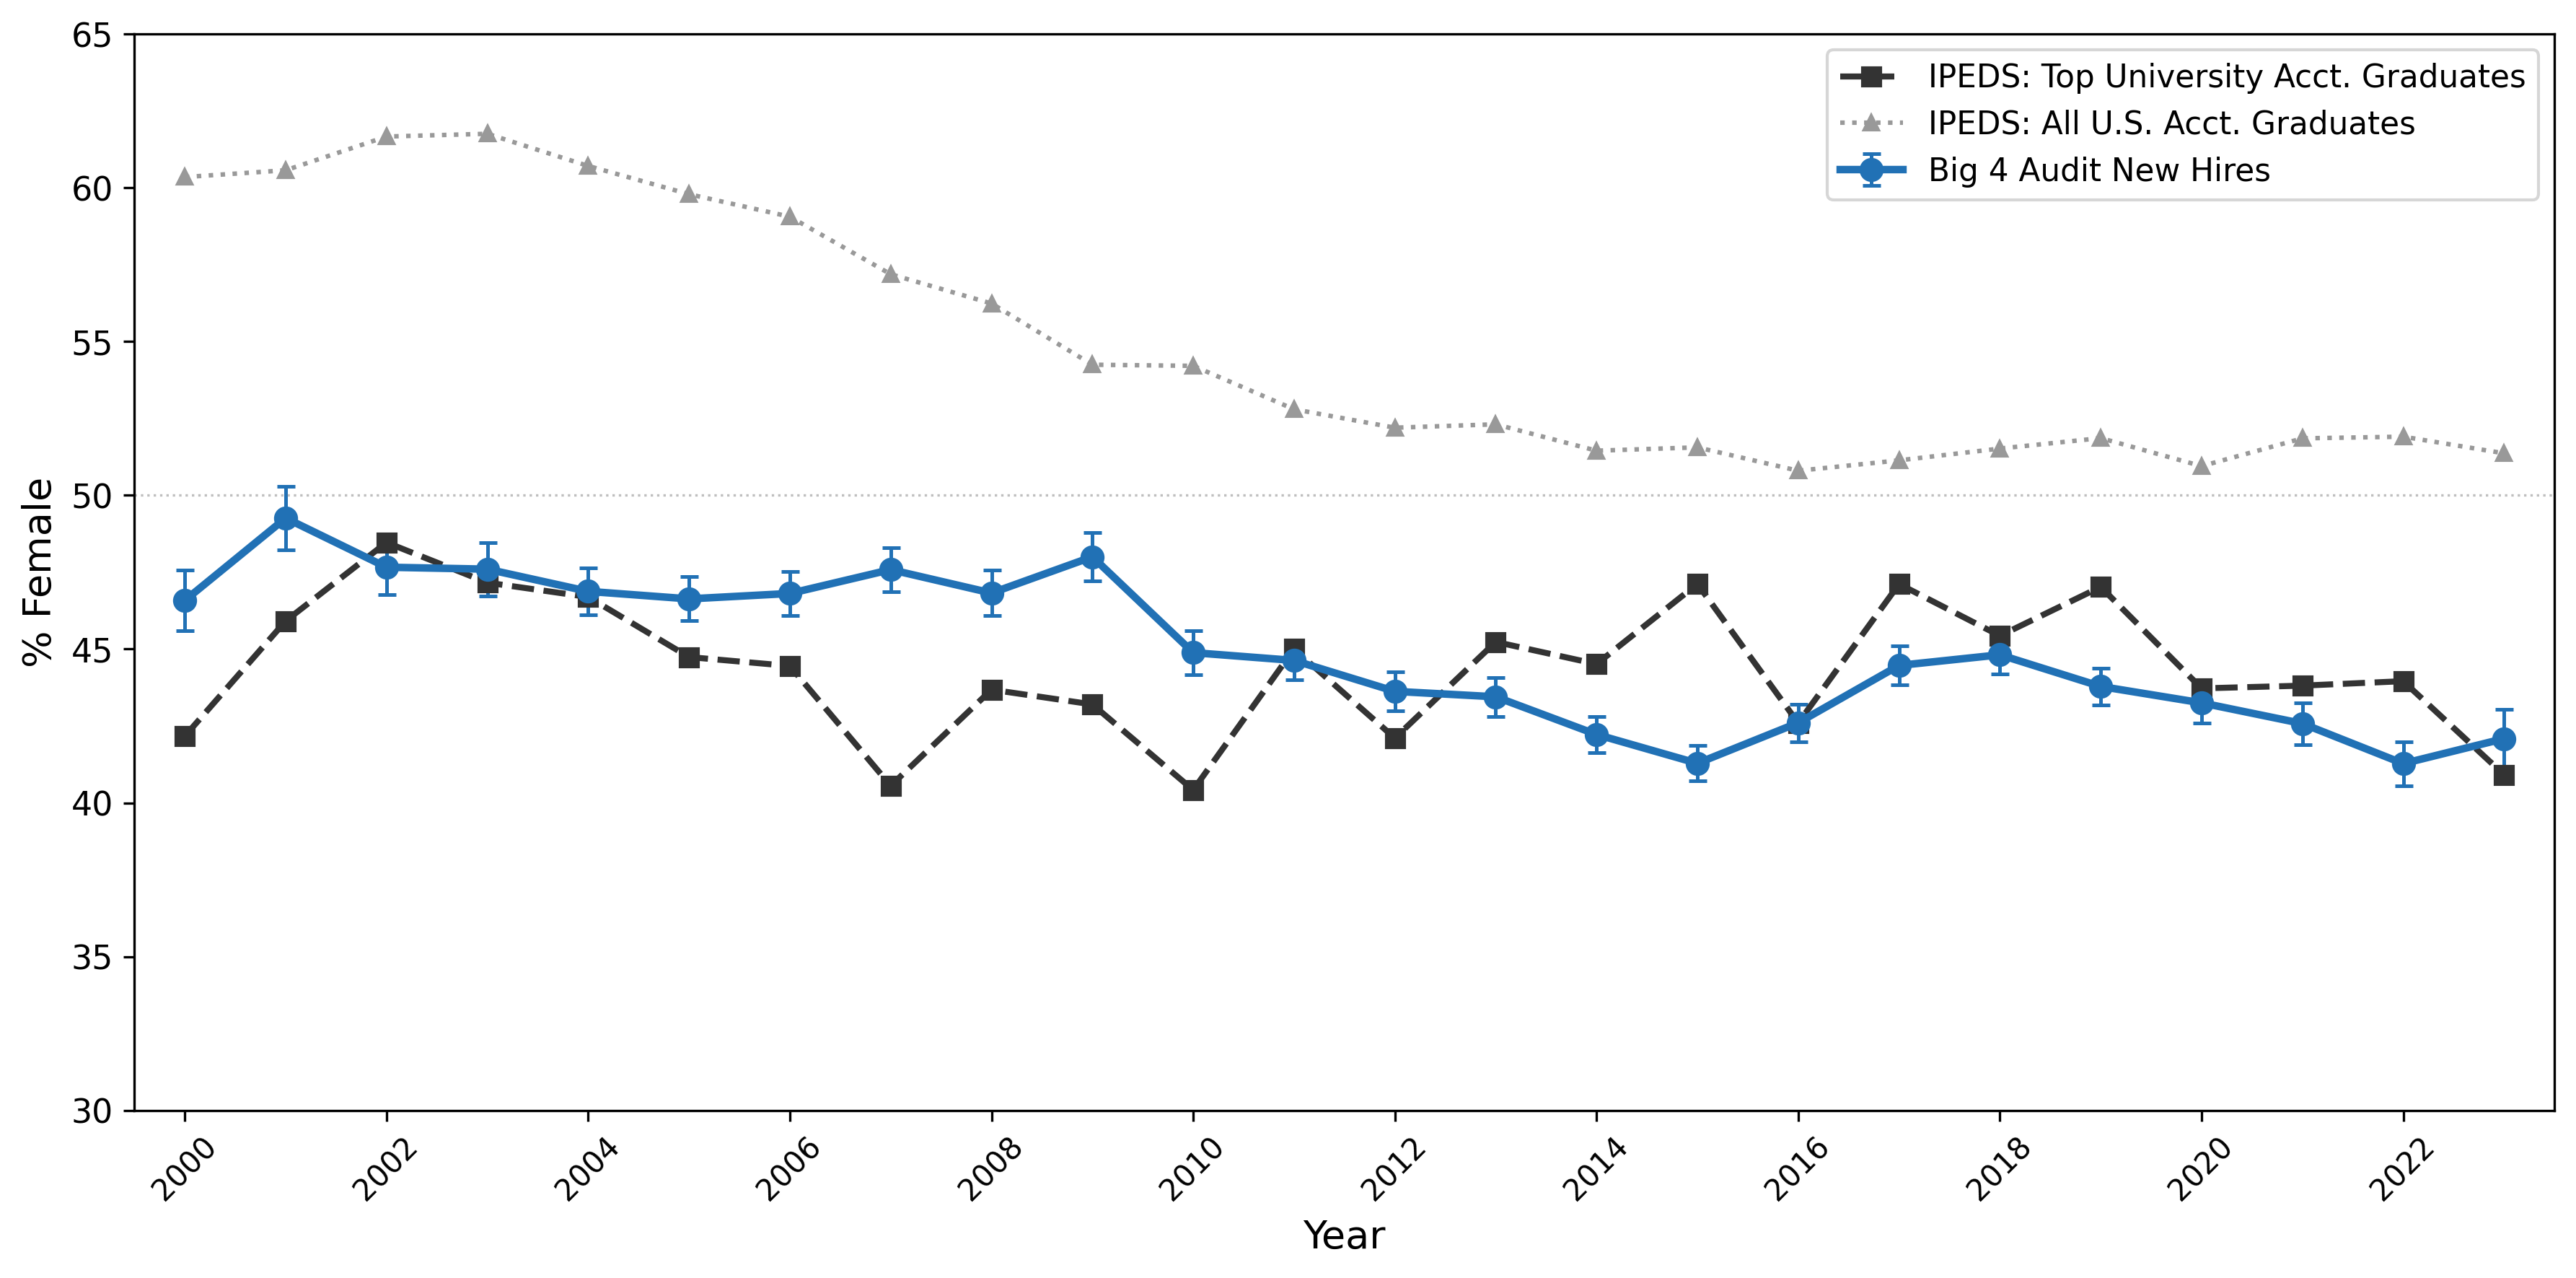
\includegraphics[width=.99\linewidth]{Figures/supplyVsEntry.png}
    \label{figure:supplyVsEntry}
    \footnotesize
    \floatfoot{\textbf{Note}: This figure compares the female share of Big~4 audit new hires (blue, with standard error bars) to the accounting talent pipeline measured using IPEDS bachelor's degree completion data. The dashed black line shows graduates from the 24 top universities used to construct our \TOPUNIVERSITY\ control variable (drawn from U.S.\ News \& World Report rankings, as listed in \textcite{FGH2022}). Results are nearly identical when restricted to the top 10 accounting programs, as the remaining universities on the list graduate relatively few accounting majors. The dotted gray line shows all U.S.\ accounting bachelor's graduates.}
\end{figure}

%----- Sample Design Table -----%
\clearpage

\clearpage
\begin{landscape}
\begin{table}[!htbp]
\begin{flushleft}
    \begin{threeparttable}[b]

        \captionsetup{labelfont=bf, singlelinecheck=off, justification=raggedright, labelsep=none}
        \caption{: Sample design}

        \input{Tables/sampleDesign}

        \begin{tablenotes}
            \footnotesize
            \item \textbf{Note}: This table describes the screening process used to construct our primary analysis sample of Big~4 audit employees. Position-level data are drawn from Revelio Labs and span 1975 through 2023.
        \end{tablenotes}
        \label{table:sampleDesign}
    \end{threeparttable}
\end{flushleft}
\end{table}
\end{landscape}

%----- Summary Statistics ----%
\clearpage
\begin{landscape}
\begin{table}[!htbp]
\begin{flushleft}
    \begin{threeparttable}[b]

        \captionsetup{labelfont=bf, singlelinecheck=off, justification=raggedright, labelsep=none}
        \caption{: Gender differences in mean values}

        \input{Tables/summaryStats.tex}

        \begin{tablenotes}
            \footnotesize
            \item \textbf{Note}: This table presents sample means for the variables used in our analysis, both for the pooled sample and separately for male and female auditors. The statistical significance of differences in means between male and female auditors is indicated by p-values in the last column. Variable definitions are provided in Appendix \ref{table:variableDefinitions}.
        \end{tablenotes}
        \label{table:summaryStats}
    \end{threeparttable}
\end{flushleft}
\end{table}
\end{landscape}

%----- Female retention in Big 4 audit (11 periods) -----%
\clearpage
\begin{table}[!htbp]
\begin{flushleft}
    \begin{threeparttable}[b]

        \captionsetup{labelfont=bf, singlelinecheck=off, justification=raggedright, labelsep=none}
        \caption{: Female retention in Big 4 audit}

        \input{Tables/mainB4Table}

        \begin{tablenotes}
            \footnotesize
            \item \textbf{Note}: This table presents OLS estimates of the effect of gender on year-to-year retention among Big~4 auditors. The dependent variable is an indicator equal to one if the auditor remains at the same firm in the following year. The key regressors are \textit{Female} $\times$ biennial period interactions spanning the full sample period; all periods are included (there is no omitted reference period). Standard errors, clustered by employee, are presented in parentheses beside each coefficient. Fixed effects for each model are indicated using the following symbols: C = entry-cohort-year, Y = calendar-year, E = employer. Sample sizes may differ across columns due to dropped singleton observations or missing values. The symbols *, **, and *** indicate p-values of \textless\, .10, \textless\, .05, and \textless\, .01 respectively. Variable definitions are provided in Appendix \ref{table:variableDefinitions}.
        \end{tablenotes}
        \label{table:mainB4}
    \end{threeparttable}
\end{flushleft}
\end{table}

% Tables 4 (promotion) and 5 (equalized family leave) removed from manuscript.
% Underlying .tex files (promotionModels.tex, eqFamModels.tex) are preserved.

%----- Mechanisms: client-side explanations -----%
\clearpage
\begin{landscape}
\begin{table}[!htbp]
\begin{flushleft}
    \begin{threeparttable}[b]

        \captionsetup{labelfont=bf, singlelinecheck=off, justification=raggedright, labelsep=none}
        \caption{: Mechanisms}

        \footnotesize
        \input{Tables/mechanismsTable}

        \begin{tablenotes}
            \footnotesize
            \item \textbf{Note}: This table presents OLS estimates of the retention model from Table~\ref{table:mainB4}, augmented with mechanism variables. Columns~1--3 each include one mechanism interaction individually. Column~4 includes all three interactions jointly. \textit{AC Female~\%} is the share of female audit committee members at the auditor's clients, aggregated to the office-year level. \textit{Gender Keywords} is the mean count of gender-related words in clients' proxy statements, aggregated to the office-year level. \textit{Post Form~AP} is an indicator for years on or after 2015. Sample sizes vary across columns because the mechanism variables are not available for all observations: \textit{AC Female~\%} requires a match between Audit Analytics engagement data and BoardEx director data, and \textit{Gender Keywords} requires a match to SEC proxy statements filed by the auditor's clients. Column~3 uses the full primary sample because \textit{Post Form~AP} is defined for all observations. Column~4 is restricted to observations for which both \textit{AC Female~\%} and \textit{Gender Keywords} are non-missing. Standard errors are clustered by employee and presented in parentheses. Fixed effects: C~=~entry-cohort-year, Y~=~calendar-year, E~=~employer. *, **, and *** indicate p-values of \textless\,.10, \textless\,.05, and \textless\,.01 respectively. Variable definitions are provided in Appendix~\ref{table:variableDefinitions}.
        \end{tablenotes}
        \label{table:mechanisms}
    \end{threeparttable}
\end{flushleft}
\end{table}
\end{landscape}

%----- Destination outcomes for Big 4 leavers -----%
\clearpage
\begin{table}[!htbp]
\begin{flushleft}
    \begin{threeparttable}[b]

        \captionsetup{labelfont=bf, singlelinecheck=off, justification=raggedright, labelsep=none}
        \caption{: Destination outcomes for Big 4 leavers}

        \input{Tables/destinationQualityPost}

        \begin{tablenotes}
            \footnotesize
            \item \textbf{Note}: This table tests whether the post-Form~AP improvement in female retention reflects constrained outside options by examining the quality of post-Big~4 destinations for auditors who leave. The sample consists of Big~4 auditors who leave the Big~4 and are observed in a subsequent position. Column~1 uses salary percentage change (next job relative to final Big~4 salary) as the dependent variable. Column~2 uses the log of days between the end of the Big~4 position and the start of the next position. \textit{Female} $\times$ \textit{Post Form AP} captures differential changes in these outcomes for female leavers after the Form AP disclosure requirement took effect. Because each observation represents one leaver, heteroskedasticity-robust standard errors are presented in parentheses beside each coefficient. Fixed effects for each model are indicated using the following symbols: F = Big~4 firm, Y = calendar-year, C = entry-cohort-year. The symbols *, **, and *** indicate p-values of \textless\, .10, \textless\, .05, and \textless\, .01 respectively. Variable definitions are provided in Appendix \ref{table:variableDefinitions}.
        \end{tablenotes}
        \label{table:leavers}
    \end{threeparttable}
\end{flushleft}
\end{table}

%----- Retention & promotion by rank (triple interaction) -----%
\clearpage
\begin{table}[!htbp]
\begin{flushleft}
    \begin{threeparttable}[b]

        \captionsetup{labelfont=bf, singlelinecheck=off, justification=raggedright, labelsep=none}
        \caption{: Female retention and promotion by audit rank}

        \input{Tables/rankInteraction}

        \begin{tablenotes}
            \footnotesize
            \item \textbf{Note}: This table presents the results of a pooled model with \FEMALE\ $\times$ Post Form~AP $\times$ Rank triple interactions, estimated on the rank subsample described in Table~\ref{table:sampleDesign} (auditors for whom we can reliably infer historical ranks). Column 1 uses \RETAINED\ as the dependent variable; Column 2 uses \PROMOTED\ (conditional on retention, excluding partners, which further reduces the sample). Because the rank indicators are exhaustive, the \FEMALE\ $\times$ Post Form~AP two-way interaction is subsumed by the three triple interactions and is not separately identified. The remaining constituent two-way interactions (Post Form~AP $\times$ Rank) and standalone terms (\FEMALE, Post Form~AP, Rank indicators, time in rank), as well as the control variables from Table~\ref{table:mainB4}, are included in each specification but their coefficients are not tabulated for parsimony. The ``Post-period net female gap'' panel reports the linear combination of the triple and two-way \FEMALE\ $\times$ Rank interaction coefficients (via Stata's \textit{lincom} command), representing the total post-Form~AP female retention or promotion differential at each rank. Standard errors, clustered by employee, are presented in parentheses beside each coefficient. Fixed effects for each model are indicated using the following symbols: C = entry-cohort-year, Y = calendar-year, E = employer. The symbols *, **, and *** indicate p-values of \textless\, .10, \textless\, .05, and \textless\, .01 respectively. Variable definitions are provided in Appendix~\ref{table:variableDefinitions}.
        \end{tablenotes}
        \label{table:rankInteraction}
    \end{threeparttable}
\end{flushleft}
\end{table}

%----- Robustness specifications -----%
\clearpage
\begin{table}[!htbp]
\begin{flushleft}
    \begin{threeparttable}[b]

        \captionsetup{labelfont=bf, singlelinecheck=off, justification=raggedright, labelsep=none}
        \caption{: Robustness tests}

        \input{Tables/robustnessModels.tex}

        \begin{tablenotes}
            \footnotesize
            \item \textbf{Note}: This table presents two robustness tests of the primary retention model from Table~\ref{table:mainB4}. Column 1 re-estimates the model as a Cox proportional hazard model instead of OLS; entry-cohort-year fixed effects are omitted because the Cox model itself accounts for duration dependence. Column 2 adds metropolitan area-by-year fixed effects to the OLS model. Control variables from Table~\ref{table:mainB4} are included in all columns but not tabulated for parsimony. Column~1 reports heteroskedasticity-robust standard errors; Column~2 reports standard errors clustered by employee. Fixed effects for each model are indicated using the following symbols: C = entry-cohort-year, Y = calendar-year, E = employer, Y*M = year-by-metropolitan area. Sample sizes may differ across columns due to dropped singleton observations or missing values. The symbols *, **, and *** indicate p-values of \textless\, .10, \textless\, .05, and \textless\, .01 respectively. Variable definitions are provided in Appendix~\ref{table:variableDefinitions}.
        \end{tablenotes}
        \label{table:robustnessModels}
    \end{threeparttable}
\end{flushleft}
\end{table}

%--------------------%
%----- Appendix -----%
%--------------------%

\appendix

\renewcommand{\tablename}{Table} 
\renewcommand{\thetable}{A\arabic{table}} 
\setcounter{table}{0}

\clearpage
\Large
Appendix
\small

\singlespacing

\begin{table}[h!]
\begin{flushleft}
    \begin{threeparttable}[b]
    \captionsetup{labelfont=bf, singlelinecheck=off, justification=raggedright, labelsep=none}
    \caption{: Revelio roles used to construct the samples}
    \input{Tables/rolesTable.tex}
    \begin{tablenotes}
        \footnotesize
        \item \textbf{Note}: This table lists the values of \textit{role\_k1500} used to query Revelio's \textit{individual\_positions} table via WRDS. We reviewed all unique values of \textit{role\_k1500} and selected roles related to auditing and a set of financial service roles that provide a meaningful comparison to auditing. $\dagger$ denotes audit roles used to construct the Big~4 and non-Big~4 auditor samples. * denotes investment banking roles used to construct the BB5 investment banking sample. $\ddagger$ denotes tax roles used to construct the Big~4 tax sample.
    \end{tablenotes}
    \label{table:rolesTable}
    \end{threeparttable}
\end{flushleft}
\end{table}

\clearpage
\begin{table}[h!]
\begin{flushleft}
    \begin{threeparttable}[b]
    \captionsetup{labelfont=bf, singlelinecheck=off, justification=raggedright, labelsep=none}
    \caption{: Big 4 employer name variants in Revelio}
    \input{Tables/firmNamesTable.tex}
    \begin{tablenotes}
        \footnotesize
        \item \textbf{Note}: This table lists the values of \textit{company\_raw} used to identify Big~4 audit positions. We identified these values by examining all unique values of \textit{company\_raw} for which at least 1,000 unique employees held an audit or auditor role at some point during our sample period. We reviewed each such value to determine whether it represents a variant of the name of a Big~4 accounting firm. Some values (e.g., ``KPMG Advisory'') refer to divisions or branding variants; inclusion in this table indicates only that the employer name is mapped to a Big~4 firm and was associated with an employee that at one time held an ``audit'' or ``auditor'' role. Whether a given employee-year is classified as an auditor is determined separately by the \textit{role\_k1500} field (see Table~\ref{table:rolesTable}).
    \end{tablenotes}
    \label{table:firmNamesTable}
    \end{threeparttable}
\end{flushleft}
\end{table}

\clearpage
\begin{table}[h!]
\begin{flushleft}
    \begin{threeparttable}[b]
    \captionsetup{labelfont=bf, singlelinecheck=off, justification=raggedright, labelsep=none}
    \caption{: Largest employers in the other financial services sample}
    \input{Tables/topCompanies.tex}
    \begin{tablenotes}
        \footnotesize
        \item \textbf{Note}: This table lists the 50 companies with the most unique employees in the other financial services (OFS) sample, ranked by employee count. * denotes the five ``Bulge Bracket'' (BB5) investment banks used as a benchmark comparison group.
    \end{tablenotes}
    \label{table:employerTable}
    \end{threeparttable}
\end{flushleft}
\end{table}

\clearpage
\begin{table}[h!]
\begin{flushleft}
    \begin{threeparttable}[b]
    \captionsetup{labelfont=bf, singlelinecheck=off, justification=raggedright, labelsep=none}
    \caption{: Non-Big 4 accounting firms by PCAOB inspection status}
    \input{Tables/nonB4FirmsTable.tex}
    \begin{tablenotes}
        \footnotesize
        \item \textbf{Note}: This table lists the non-Big~4 accounting firms identified from the \textit{Accounting Today} Top~100 rankings and matched to Revelio employment records. Panel~A lists firms subject to PCAOB annual inspection, which serves as a proxy for significant Form~AP exposure. Panel~B lists firms not subject to annual inspection. Firm names reflect the most recent name where mergers or rebranding occurred during the sample period. The list contains 155 firms rather than 100 because the \textit{Accounting Today} rankings change over time as firms merge, rebrand, or enter and exit the list; the 155 firms represent the cumulative set of distinct firms that appeared in the rankings between 1998 and 2025. Each firm was matched to Revelio's \textit{company\_raw} field by identifying all name variants associated with the firm, resulting in 725 unique \textit{company\_raw} values. The individual \textit{company\_raw} values are available from the authors upon request.
    \end{tablenotes}
    \label{table:nonB4Firms}
    \end{threeparttable}
\end{flushleft}
\end{table}

\clearpage
\begin{flushleft}
\input{Tables/VariableDefinitions.tex}
\end{flushleft}

%-----------------------------%
%----- Internet Appendix -----%
%-----------------------------%
% \clearpage
% \input{Sections/InternetAppendix}

\end{document}
